%    minted language=cpp,

%%%%%%
%%%%%%%%%%%%%%%%%%%%%%%%%%%%%% Title Page Info %%%%%%%%%%%%%%%%%%%%%%%%%%%%%%%%%%%%%%%%%%%
%%%%%%%%%%%%%%%%%%%%%%%%%%%%%%%%%%%%%%%%%%%%%%%%%%%%%%%%%%%%%%%%%%%%%%%%%%%%%%%%%%%%%%%%%%

\documentclass[aspectratio=169,compress]{beamer}
\mode<presentation> 

\usetheme{Warsaw}
\usecolortheme[rgb={0.7,0.0,0.0}]{structure}


\usepackage[algosection,lined]{algorithm2e}
\usepackage{minted}
\usepackage{tcolorbox}
\tcbuselibrary{minted}


% define
%\usepackage{beamerouterthememiniframes} % Para los puntitos 
\setbeamertemplate{footline}[frame number]{}

% include packages
\usepackage{subfigure}
\usepackage{multicol}
\usepackage{amsmath}
\usepackage{epsfig}
\usepackage{graphicx}
\usepackage[all,knot]{xy}
\usepackage{algorithmic}
\xyoption{arc}
\usepackage{url}
\usepackage{multimedia}
\usepackage{hyperref}
\usepackage{tikz}

\usepackage{pgfpages}
\setbeameroption{hide notes} % Only slides
%\setbeameroption{show only notes} % Only notes
%\setbeameroption{show notes on second screen=right} % Both



\usepackage{minted}
\usepackage{tcolorbox}
\tcbuselibrary{minted}


%\title{20 proyectos de la línea de sistemas inteligentes de la maestría en ingeniería de la UPV: aplicaciones en el área de salud, agroindustria, seguridad y educación}
%\title{Proyectos selectos de visión por computadora y aprendizaje automático del Laboratorio de Sistemas Inteligentes de la UPV} % TecMTY
\title{Fundamentos de VR-AR mediante aplicaciones Gráficas 3D en Android utilizando OpenGL- Parte II\\ \large 3er Foro Nacional de Tecnologías de la Información y Sistemas Computacionales} % UPP

\author{Dr. Marco Aurelio Nu\~no Maganda}
\institute{Universidad Politécnica de Victoria\\ Laboratorio de Sistemas Inteligentes \\
mnunom@upv.edu.mx  \vspace{.25cm} }

\date{28 y 29 de Septiembre de 2023}


%%%%%%%%%%%%%%%%%%%%%%%%%%%%%%%%%%%%%%%%%%%%%%%%%%%%%%%%%%%%%%%%%%%%%%%%%%%%%%%%%%%%%%%%%%
%%%%%%%%%%%%%%%%%%%%%%%%%%%%%% Begin Your Document %%%%%%%%%%%%%%%%%%%%%%%%%%%%%%%%%%%%%%%
%%%%%%%%%%%%%%%%%%%%%%%%%%%%%%%%%%%%%%%%%%%%%%%%%%%%%%%%%%%%%%%%%%%%%%%%%%%%%%%%%%%%%%%%%%

 

\usepackage[backend=biber,maxcitenames=50,maxbibnames=50,sorting=ydmdddnt]{biblatex}

\DeclareSortingScheme{ydmdddnt}{ 
  \sort{ 
    \field{presort} 
  } 
  \sort[final]{ 
    \field{sortkey} 
  } 
  \sort[direction=descending]{ 
    \field{year} 
  } 
  \sort[direction=descending]{ 
    \field{month} 
  } 
  \sort[direction=descending]{ 
    \field{day} 
  } 
  \sort{ 
    \field{journaltitle} 
  } 
  \sort{ 
    \field{author} 
    \field{editor} 
  } 
  \sort{ 
    \field{title} 
  } 
}




%\renewrobustcmd{\mkbibfootnote}{\normalsize\footnotemark\footnotetext}
\setbeamerfont{footnote}{size=\tiny}


% Articulo de Brujano-
\newcommand{\CitaA}{MarcoNuno_CongArbEsp_2013_11_01}
\newcommand{\CitaB}{Reporte2019}

%\newcommand{\CitaB}{MarcoNuno_CongArbEsp_2004_09_00}
\newcommand{\CitaC}{MarcoNuno_CongArbIng_2005_09_00}
\newcommand{\CitaD}{MarcoNuno_CongArbIng_2009_06_00}
\newcommand{\CitaE}{MarcoNuno_CongArbIng_2010_12_00}
\newcommand{\CitaF}{MarcoNuno_Revista_2011_06_00}
\newcommand{\CitaG}{MarcoNuno_CongArbIng_2011_08_00}
\newcommand{\CitaH}{MarcoNuno_CongArbIng_2011_10_00}
\newcommand{\CitaI}{MarcoNuno_CongArbIng_2012_08_00}
\newcommand{\CitaJ}{MarcoNuno_Revista_2012_09_00}
\newcommand{\CitaK}{MarcoNuno_CongArbIng_2014_02_00}
\newcommand{\CitaL}{MarcoNuno_CongArbIng_2014_06_00}
\newcommand{\CitaM}{8994792} %Articulo de Antonio...


\newcommand{\ArchivoPrincipal}{Todos}
\newcommand{\ArchivoSecundario}{Bibliografia}
\newcommand{\ArchivoTerciario}{SinPublicar}


%Append keywords to identify different bibliography entries.
\DeclareSourcemap{
  \maps[datatype=bibtex, overwrite]{
    \map{
      \perdatasource{\ArchivoPrincipal.bib}
      \step[fieldset=KEYWORDS, fieldvalue=primary, append]
    }
    \map{
      \perdatasource{\ArchivoTerciario.bib}
      \step[fieldset=KEYWORDS, fieldvalue=primary, append]
    }
    \map{
      \perdatasource{\ArchivoSecundario.bib}
      \step[fieldset=KEYWORDS, fieldvalue=secundary, append]
    }    
  }
}


\addbibresource{\ArchivoPrincipal.bib}
\addbibresource{\ArchivoSecundario.bib}
\addbibresource{\ArchivoTerciario.bib}





\newcommand{\markedsection}[2]{\section[#2]{#2%
\sectionmark{#1}}
\sectionmark{#1}}

\newcommand{\markedsubsection}[2]{\subsection[#2]{#2%
\subsectionmark{#1}}
\subsectionmark{#1}}


\newcommand{\Titulo}{""}
\newcommand{\SectionTitle}{""}

\AtBeginSection[]
{
    \begin{frame}
        \frametitle{Outline}
        \tableofcontents[currentsection]
    \end{frame}
}



\begin{document}
%\logo{
\includegraphics[width=3cm]{FigsOpenGL/LogoUPV}\hspace*{9cm}~%
%  
\includegraphics[width=3cm]{FigsOpenGL/LogoUPV}
%}
\frame{
	%\titlepage 
	\begin{titlepage}
	\end{titlepage}
	
}
%\logo{}





%% Fuentes potenciales:
% https://stuff.mit.edu/afs/sipb/project/android/docs/training/graphics/opengl/index.html
% https://github.com/huntto/android-opengles-2.0
% Android and OpenGL
% https://github.com/zperkowski/DoomGLes

\section[Intro]{OpenGL, GLSL y tecnologías asociadas}




% https://www.mathematik.uni-marburg.de/~thormae/lectures/graphics1/graphics_4_1_eng_web.html#1
\frame{
\frametitle{OpenGL}
\begin{itemize}
\item OpenGL significa Open Graphics Library, un estándar para la progamación gráfica.
\item Los comandos de gráficos son implementados por el controlador de la tarjeta gráfica y, por lo tanto, son independientes del hardware de la tarjeta gráfica, del sistema operativo y del administrador de ventanas empleado.
\item Los comandos de gráficos están cercanos hardware y son suficientes para lograr la funcionalidad principal
\item Varias bibliotecas y frameworks se basan en OpenGL y permiten la programación a un mayor nivel de abstracción.
\end{itemize}
}

\frame{
\frametitle{Versiones OpenGL para PC}
\begin{itemize}
\item Desde su introducción (1992) OpenGL se ha ampliado continuamente para admitir nuevas funciones de tarjetas gráficas.
\item OpenGL 1.0 (1992), OpenGL 1.1 (1997), OpenGL 1.2 (1998), OpenGL 1.3 (2001), OpenGL 1.4 (2002), OpenGL 1.5 (2003)
\item OpenGL 2.0 (2004), OpenGL 2.1 (2006)
\item OpenGL 3.0 (2008), OpenGL 3.1 (2009), OpenGL 3.2 (2009), OpenGL 3.3 (2010)
\item OpenGL 4.0 (2010), OpenGL 4.1 (2010), OpenGL 4.2 (2011), OpenGL 4.3 (2012), OpenGL 4.4 (2013), OpenGL 4.5 (2014), OpenGL 4.6 (2017)
%\item En esta ponencia, se combina la versi
\item A partir de la  versión 3.1, el Pipeline de funciones fijo ya no esta soportado, por l ocual es necesario implementar shaders, lo cual dificulta el aprendizaje.
\end{itemize}
}


\frame{
\frametitle{OpenGL ES y WebGL}
\begin{itemize}
\item OpenGL ES (Embedded System) es una versión de OpenGL con funcionalidad reducida para teléfonos móviles, televisores, tabletas, etc.
\item OpenGL ES 1.0 (2003): similar a OpenGL 1.3 (Pipeline Fijo)
\item OpenGL ES 1.1 (2004): similar a OpenGL 1.5 (compatible con versiones anteriores)
\item OpenGL ES 2.0 (2007): similar a OpenGL 2.0 (no compatible con versiones anteriores)
\item OpenGL ES 3.0 (2012): similar a OpenGL 3.3 
\item OpenGL ES 3.1 (2014): similar a OpenGL 4.3
\item OpenGL ES 3.2 (2015): similar a OpenGL 4.3
\item OpenGL ES 3.3 (2017): similar a OpenGL 4.6
\item WebGL esta basado en OpenGL ES 2.0 (y WebGL 2.0 en OpenGL ES 3.0) y permite gráficos 3D en páginas web (compatible con la mayoría de navegadores)
\end{itemize}
}

\begin{frame}{SoCs para Teléfonos Inteligentes}
\begin{columns}
\begin{column}{0.60\textwidth}  
\begin{itemize}
\item El término SoC significa system-on-a-chip.
\item Un SoC es un sistema completo contenido en un solo circuito integrado.
\item La combinación de todos sus componentes en una sola unidad de procesamiento permite un ahorro de energía significativo. 
\item Bloques comunes en un SoC:
\begin{itemize}
\item Central Processing Unit (CPU).
\item Graphics Processing Unit (GPU).
\item Image Processing Unit (ISP).
\item Digital Signal Processor (DSP).
\item Neural Processing Unit (NPU).
\item Video encoder/decoder.
\item Modems.
\end{itemize}
\end{itemize}
\end{column}
\begin{column}{0.40\textwidth}  
    \begin{center}
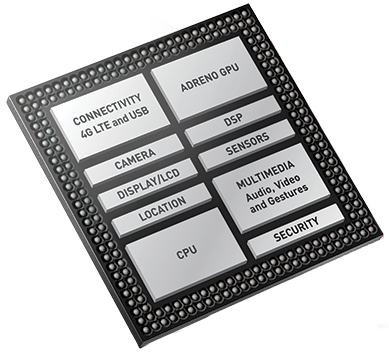
\includegraphics[width=0.65\textwidth]{FigsOpenGL/qualcomm_snapdragon410_block}\\
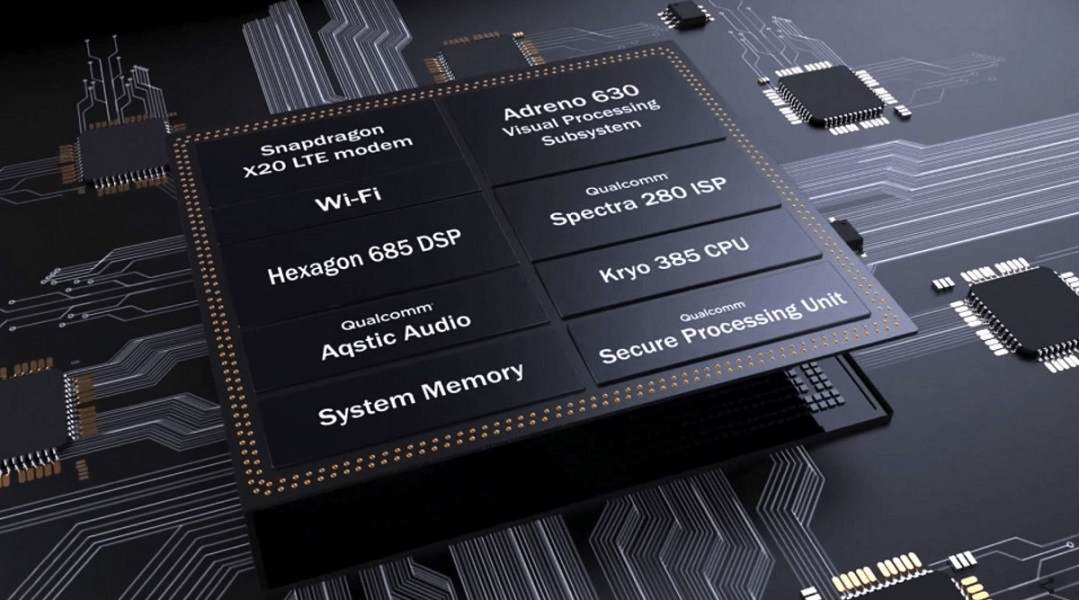
\includegraphics[width=0.85\textwidth]{FigsOpenGL/Snapdragon-855-1}
     \end{center}
\end{column}
\end{columns}
\end{frame}


\frame{
\frametitle{¿Qué es un GPU (Graphics Processing Unit)?}
\begin{columns}
\begin{column}{0.49\textwidth}
\begin{itemize}
\item Un GPU es un procesador formado por muchos núcleos más pequeños y especializados, especializada en operaciones de punto flotante en paralelo.
\item Al trabajar conjuntamente, los núcleos ofrecen un desempeño masivo cuando se puede dividir una tarea de procesamiento y es procesada por muchos núcleos.
\item Por ejemplo, el Samsung S10 utiliza un Qualcomm Snapdragon 855 SoC (tiene un CPU de 8 núcleos y un GPU dedidado para gráficos (Adreno 640).
\end{itemize}
\end{column}
\begin{column}{0.19\textwidth}
\begin{center}
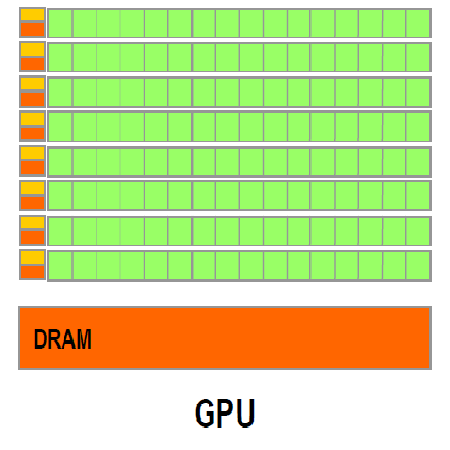
\includegraphics[width=0.9\textwidth]{FigsOpenGL/GPU}\\
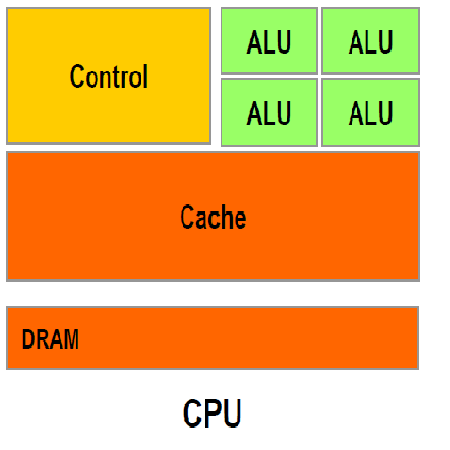
\includegraphics[width=0.9\textwidth]{FigsOpenGL/CPU}\\
\end{center}
\end{column}
\begin{column}{0.30\textwidth}  
    \begin{center}
     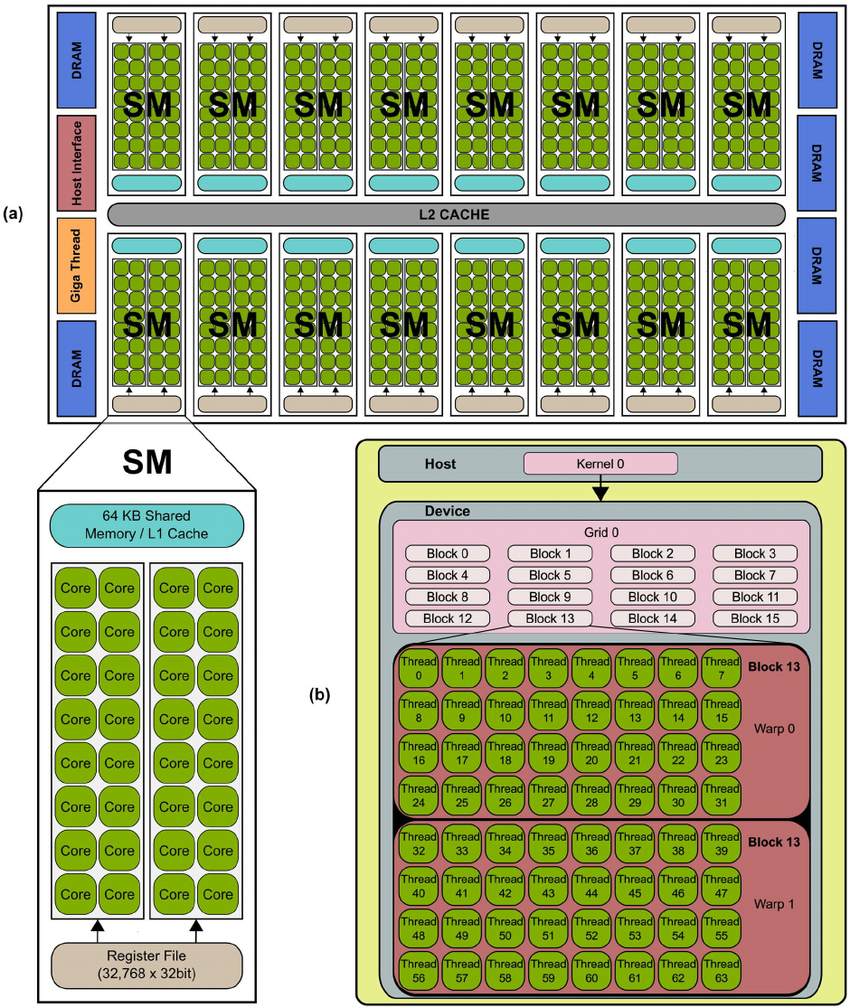
\includegraphics[width=\textwidth]{FigsOpenGL/Typical-NVIDIA-GPU-architecture}
     \end{center}
\end{column}
\end{columns}
}



%\begin{frame}{OpenGL}
%OpenGL signfiica Open Graphics Library, un estándar para la progamación de gráfica.
%El OpenGL Shading Language es un lengauje de alto nivel (cuya sintaxis es parecida a C) diseñado para procesamiento en paralelo en un GPU. 
%\end{frame}



\begin{frame}{OpenGL Pipeline}

\begin{columns}
\begin{column}{0.45\textwidth}
\begin{itemize}
\item Un Pipeline es una estructura de procesamiento paralelo
\item Un GPU tiene dos tipos de procesadores, incorporados en un Pipeline:
\begin{itemize}
\item El vertex processor
\item El fragment processor
\end{itemize}
\item Los programas son cargados en cada procesador.
\end{itemize}
\end{column}
\begin{column}{0.45\textwidth}
    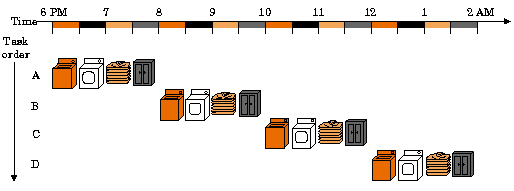
\includegraphics[width=\textwidth]{FigsOpenGL/Pipeline1.png}\\
    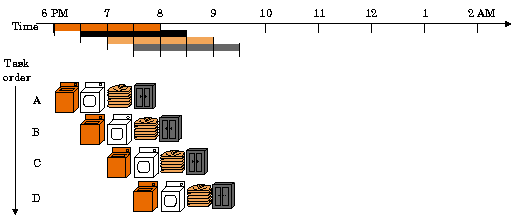
\includegraphics[width=\textwidth]{FigsOpenGL/Pipeline2.png}    
\end{column}
\end{columns}

\end{frame}


\begin{frame}{OpenGL Pipeline (2)}
    \begin{center}
    %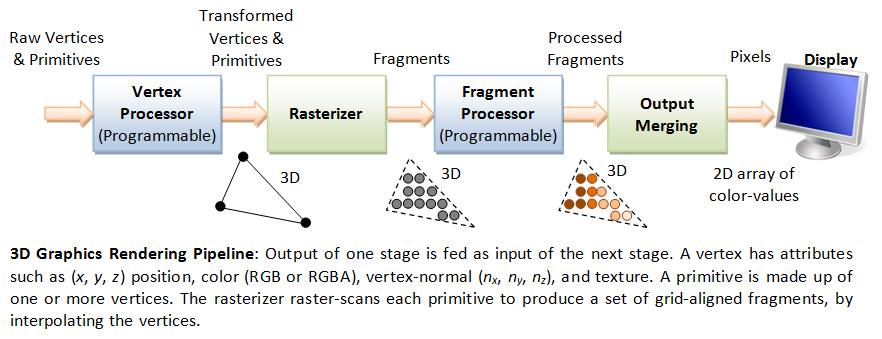
\includegraphics[width=\textwidth]{FigsOpenGL/Graphics3D_Pipe}
    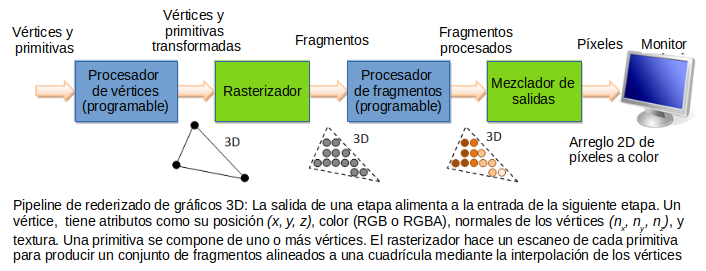
\includegraphics[width=\textwidth]{FigsOpenGL/OpenGL_Pipeline_Espaniol.png}
    \end{center}
\end{frame}


\begin{frame}{OpenGL Pipeline (3)}
    \begin{center}
    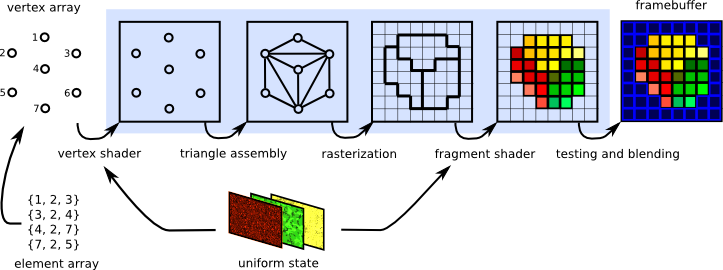
\includegraphics[width=\textwidth]{FigsOpenGL/evasgl-graphics-pipeline}
    \end{center}
\end{frame}

\begin{frame}{OpenGL Shading Language}
\begin{itemize}
\item Las aplicaciones móviles son ejecutadas principalmente en el CPU y la memoria principal
\item Para procesamiento de gráficos, los programas son ejecutados en el GPU el cual tiene su propia memoria local (memoria gráfica).
\item Los programas del GPU son escritos en un lenguaje llamado Shading Language (Lenguaje de sombreado). 
\item La mayoría de los GPUs adoptaron el lenguaje de OpenGL shading Language (OGSL)
\end{itemize}
\end{frame}

\begin{frame}{Transformaciones}
    \begin{center}
    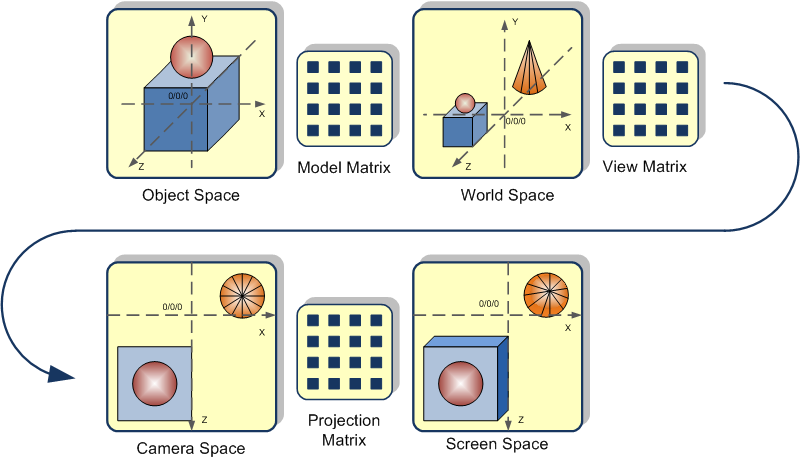
\includegraphics[width=0.75\textwidth]{FigsOpenGL/ModelViewProjection_MVP_Matrix}
    \end{center}
\end{frame}

	






\begin{frame}{Instrucciones para replicar los proyectos de este taller }
\begin{itemize}
\item Siempre crear un proyecto Android Studio nuevo, seleccionando JAVA (salvo que se indique lo contrario)
\item Poner un nombre significativo al proyecto (Puede empezar por el numero de demo, pero tambien incluir información de su funcionalidad)
\item Se provee de una carpeta en el siguiente repositorio, la cual deben descargar. Los proyectos estan ordenados de manera secuencial y todo lo necesario para generar el respectivo proyecto esta dentro de dicha carpeta.

\end{itemize}
\begin{block}{Github}
\begin{center}
\tiny
\url{https://github.com/mnunom-upv/Fundamentos-de-VR-AR-mediante-aplicaciones-Gr-ficas-3D-en-Android-utilizando-OpenGL}
\end{center}
\end{block}

\end{frame}


%\section{Shading Language}
%\begin{frame}{}
%\end{frame}

\section{Primitivas 2D}
\begin{frame}{Dibujo de Primitivas}
%\begin{itemize}
%\item Primer Demo del Imperial College (Dibujar un triangulo)
%\item ** Dibujar un Hexagono
%\item ** Explicar primitivas graficas 
%\end{itemize}
%\begin{block}{Demo \#1}
%Dibujar un Triangulo en 2D
%\end{block}
\begin{columns}
\begin{column}{0.4\textwidth}
\begin{itemize}
\item Para dibujar cualquier superficie en OpenGL, se debe triangular los vértices adyacentes para formar polígonos (generalmente triangulos).
\item Se requieren de dos triangulos para dibujar un cuadrado.
\end{itemize}


\end{column}
\begin{column}{0.3\textwidth}
\begin{center}
 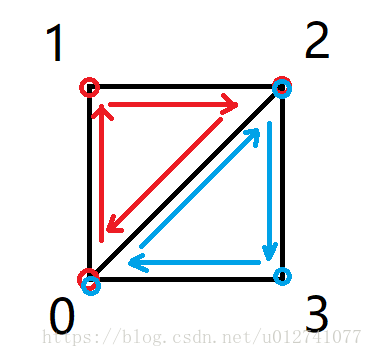
\includegraphics[width=0.98\textwidth]{FigsOpenGL/Cuadrado_Formado_por_Triangles}
 \end{center}

\end{column}
\begin{column}{0.3\textwidth}
\begin{center}
 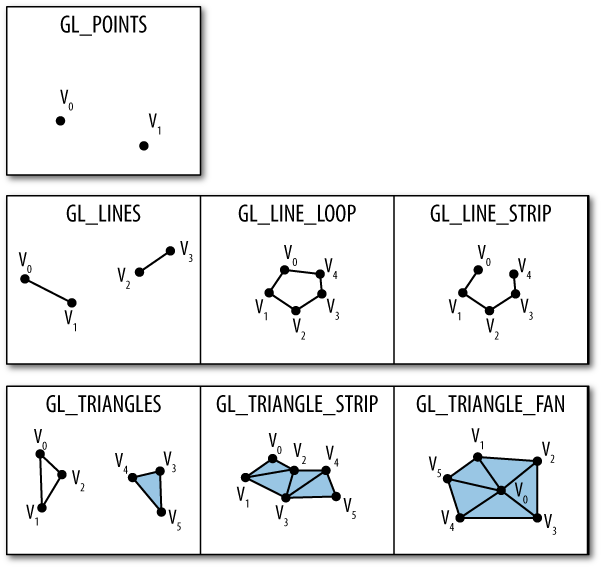
\includegraphics[width=0.98\textwidth]{FigsOpenGL/PrimitiavasOpenGL}
 \end{center}
\end{column}
\end{columns}



\end{frame}


\begin{frame}{Desplegando gráficos en 2D}

\begin{columns}
\begin{column}{0.8\textwidth}
\begin{block}{Demo \#1: Triangulo 2D en OpenGL ES}
\begin{itemize}
\item Sustituir el MainActivity.java del proyecto con el MainActivity de la carpeta del demo
\item Copiar los archivos Triangle.java, MyRenderer.java y MyView.java en la carpeta del package
%\item Copiar el archivo \textit{activity\_main.xml} a la carpeta \textit{res/layout}
\end{itemize}
\end{block}
\end{column}
\begin{column}{0.2\textwidth}
\begin{center}
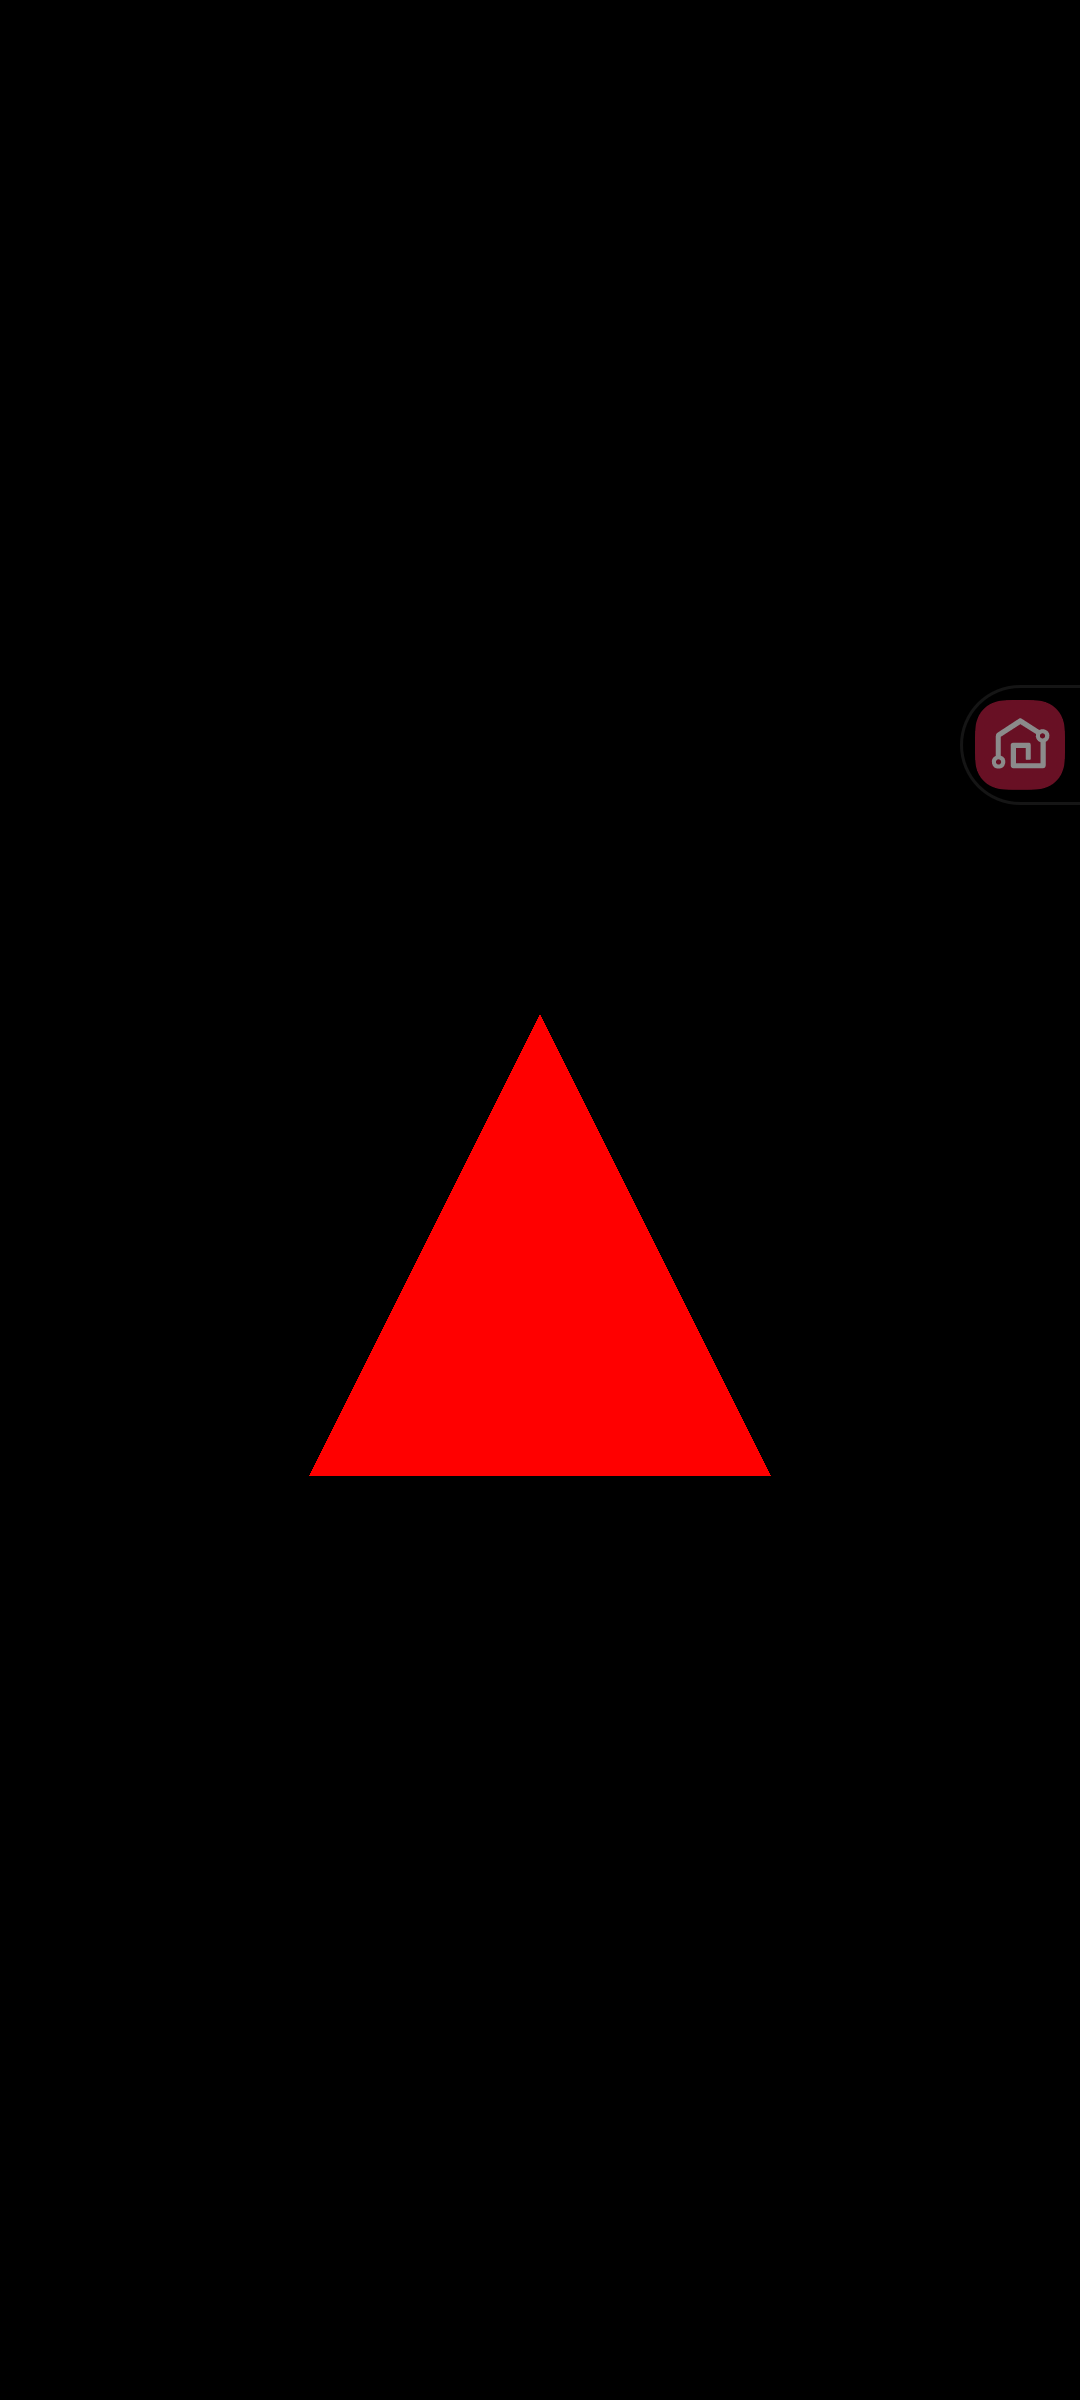
\includegraphics[width=1.0\linewidth]{PantallazosDemoTaller/Demo01.png}
\end{center}
\end{column}
\end{columns}


\end{frame}



\begin{frame}{Experimentado con Primitivas}
\begin{columns}
\begin{column}{0.5\textwidth}
\begin{itemize}
\item Es posible dibujar objetos complejos si se tiene un entendimiento correcto de las primitivas 
\item Por ejemplo: Dibujar un Hexagono Relleno/Alambrico. 
\end{itemize}
\end{column}
\begin{column}{0.5\textwidth}
\begin{center}
 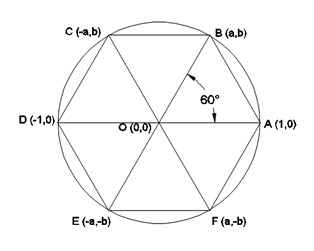
\includegraphics[width=0.98\textwidth]{FigsOpenGL/Hexagono}
 \end{center}
\end{column}
\end{columns}

\end{frame}


\begin{frame}{Desplegando gráficos en 2D}

\begin{columns}
\begin{column}{0.5\textwidth}
\begin{block}{Demo \#2: Dibujar un poligono regular de N lados empleando triángulos}
\begin{itemize}
\item Sustituir el MainActivity.java del proyecto con el MainActivity de la carpeta del demo
\item Copiar los archivos CircleFan.java, MyGLSurfaceView.java y MyGLRenderer.java en la carpeta del package
%\item Copiar el archivo \textit{activity\_main.xml} a la carpeta \textit{res/layout}
\end{itemize}
\end{block}
\end{column}
\begin{column}{0.5\textwidth}
\begin{center}
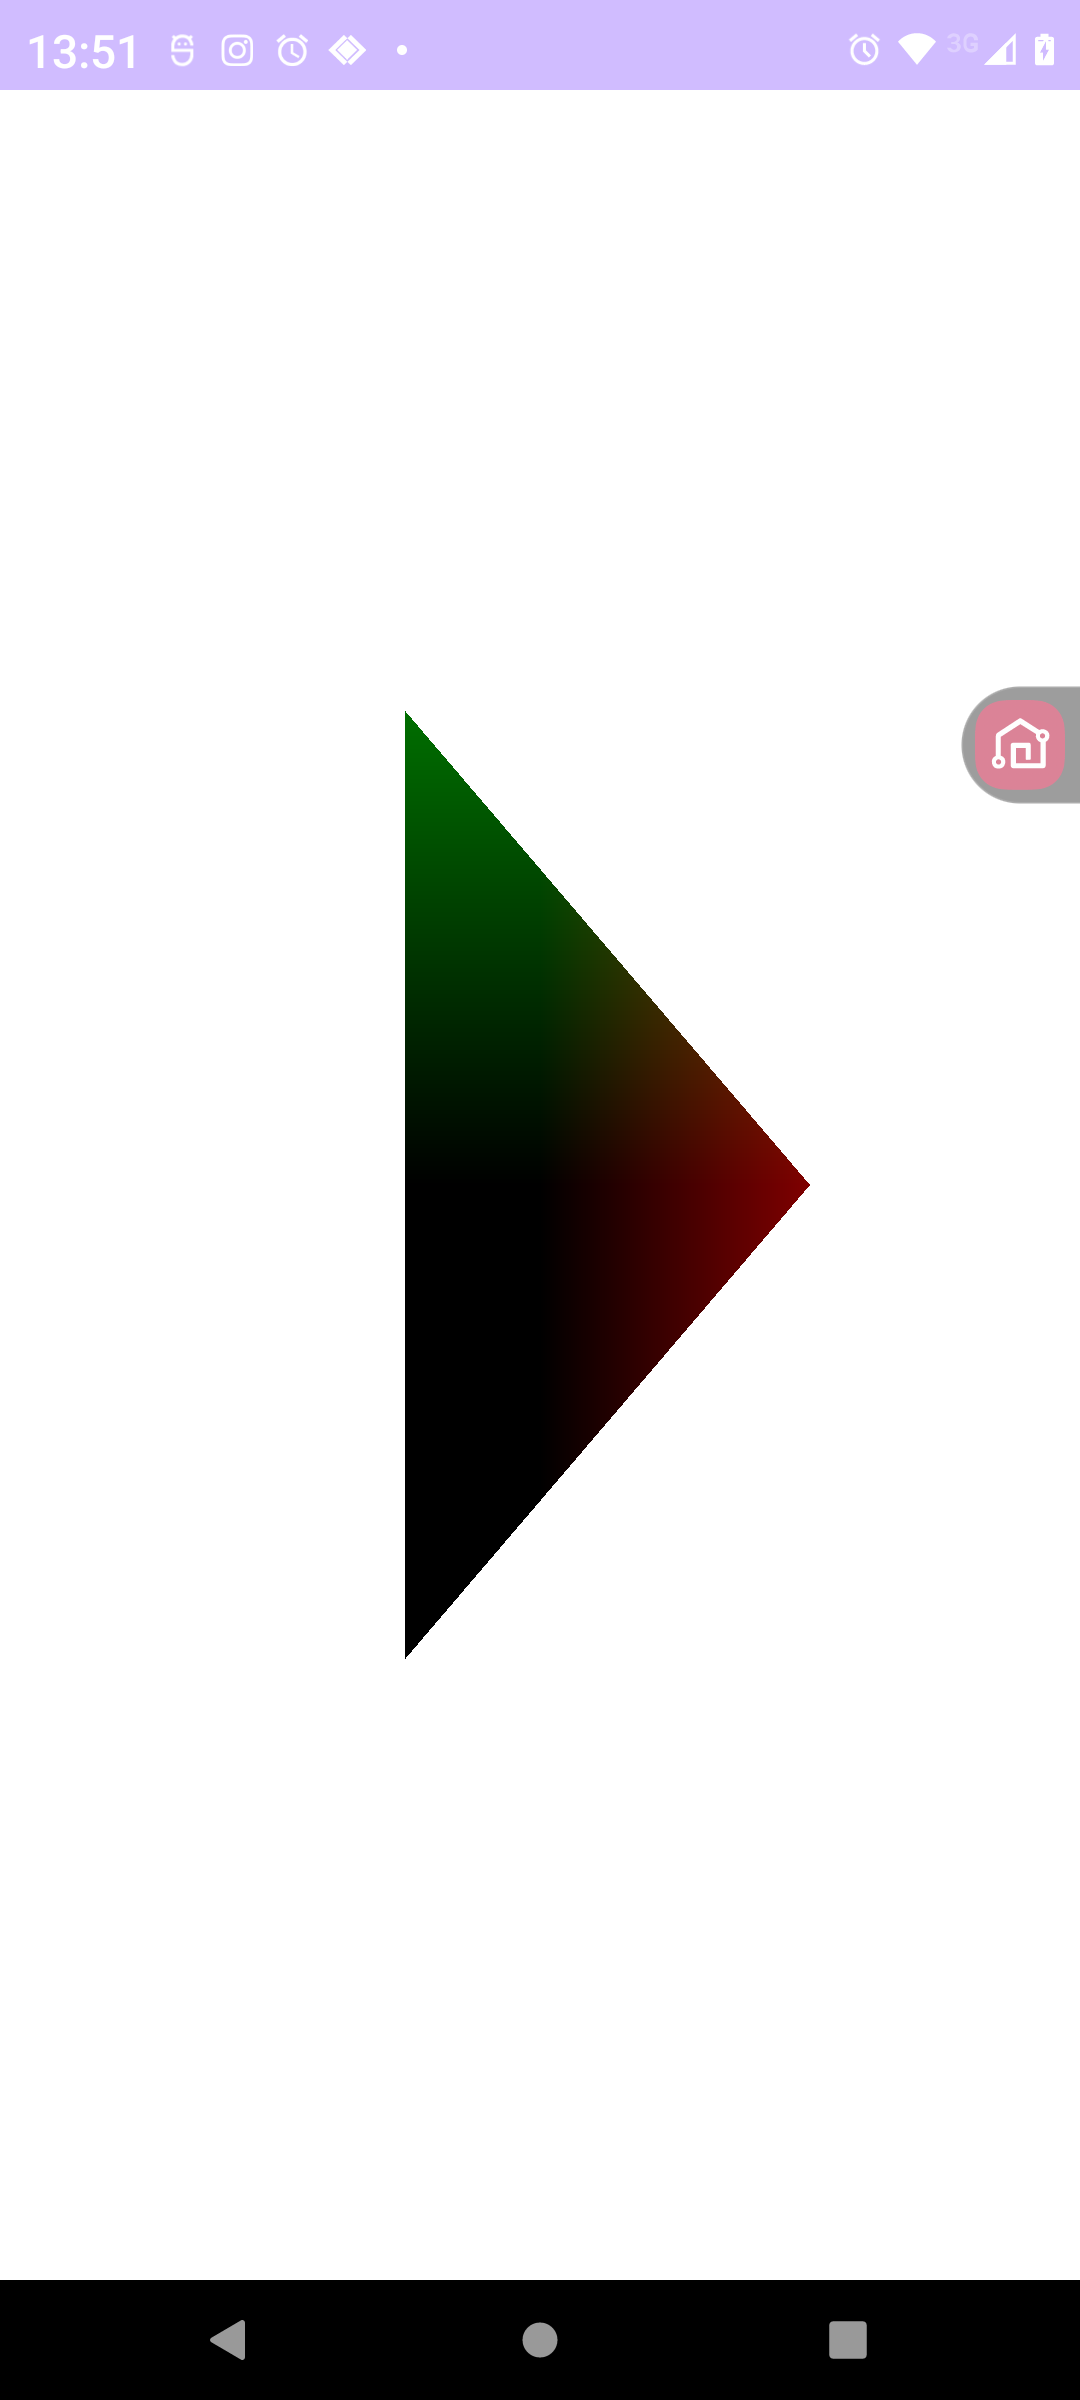
\includegraphics[width=0.35\linewidth]{PantallazosDemoTaller/Demo02-1.png}
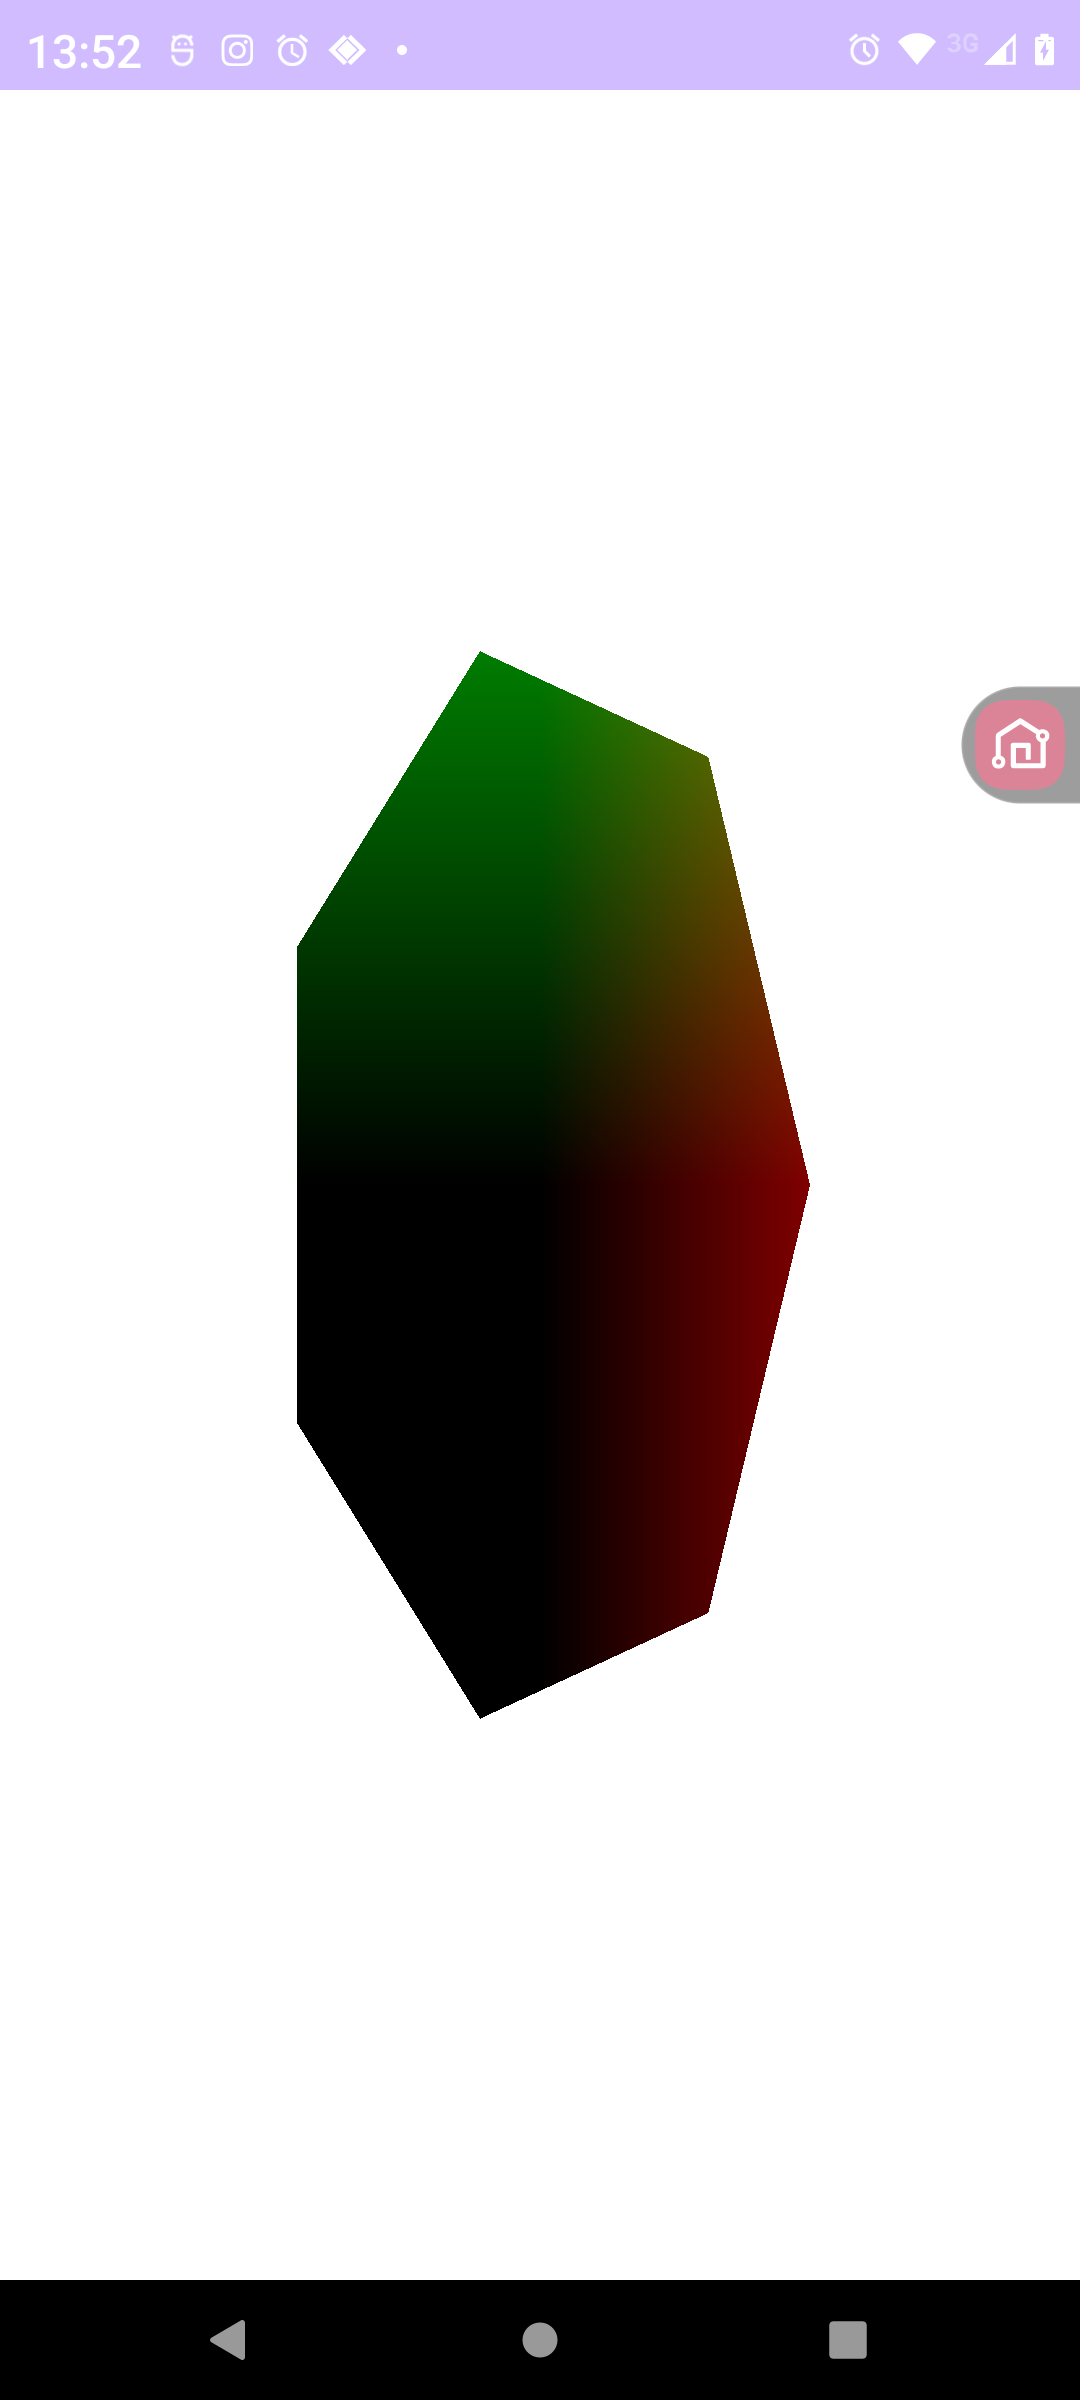
\includegraphics[width=0.35\linewidth]{PantallazosDemoTaller/Demo02-3.png}
\end{center}
\end{column}
\end{columns}


\end{frame}




\section{Primitivas 3D}
\begin{frame}{Cubo 3D}
%\begin{itemize}
%\item Lesson 00, Colored Cube
%\item Letra A
%\item Lesson 01, Transformaciones
%\item Esfera 
%\end{itemize}

\begin{columns}
\begin{column}{0.4\textwidth}



\begin{center}
 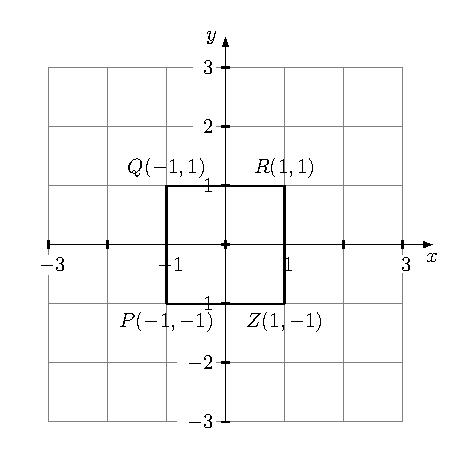
\includegraphics[width=0.98\textwidth]{FigsOpenGL/planocartersiano}
 \end{center}
\end{column}
\begin{column}{0.4\textwidth}
\begin{center}

  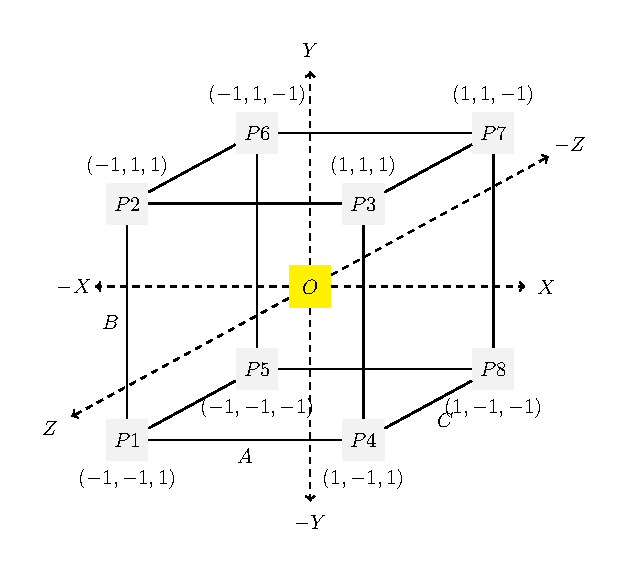
\includegraphics[width=0.98\textwidth]{FigsOpenGL/cube}
 \end{center}

\end{column}
\begin{column}{0.3\textwidth}
\begin{center}

 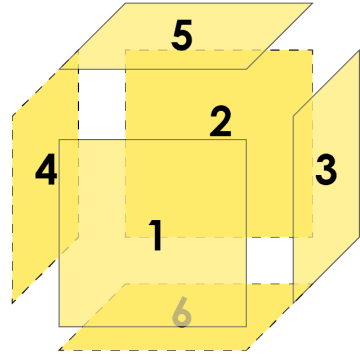
\includegraphics[width=0.98\textwidth]{FigsOpenGL/CarasCubo}
 \end{center}
\end{column}
\end{columns}

\end{frame}




\begin{frame}{Objetos 3D Complejos en OpenGL (0)}
\begin{columns}
\begin{column}{0.7\textwidth}
\begin{block}{Demo \#3: Cubo en OpenGL}
\begin{itemize}
\item Sustituir el MainActivity.java del proyecto con el MainActivity de la carpeta del demo
\item Copiar los archivos Cube.java y CubeRenderer.java en la carpeta del package
\item Copiar el archivo \textit{activity\_main.xml} a la carpeta \textit{res/layout}
\end{itemize}
\end{block}
\end{column}
\begin{column}{0.3\textwidth}
\begin{center}
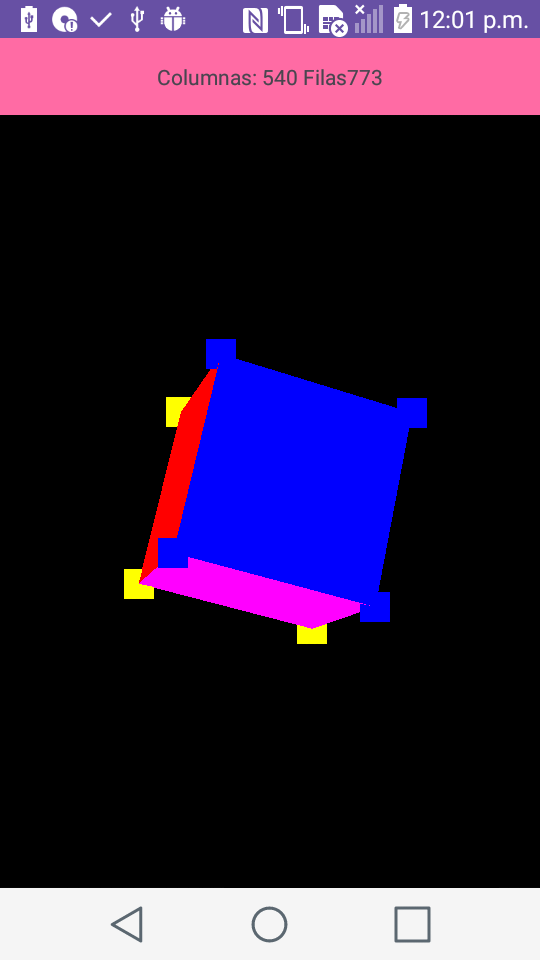
\includegraphics[width=1.0\linewidth]{PantallazosDemoTaller/Demo3.png}
\end{center}
\end{column}
\end{columns}



\end{frame}







\begin{frame}{Objetos 3D Complejos en OpenGL (1)}

\begin{columns}
\begin{column}{0.8\textwidth}
\begin{itemize}
\item Una vez que se entiende como generar las coordenadas de poligonos y asignarles un color, es posible construir objetos 3D complejos.
\end{itemize}
\begin{block}{Demo \#4: Letra A en 3D}
\begin{itemize}
\item Sustituir el MainActivity.java del proyecto con el MainActivity de la carpeta del demo
\item Copiar los archivos CharacterA.java, MyRenderer.java y MyView.java en la carpeta del package
\end{itemize}

\end{block}

\end{column}
\begin{column}{0.2\textwidth}
\begin{center}
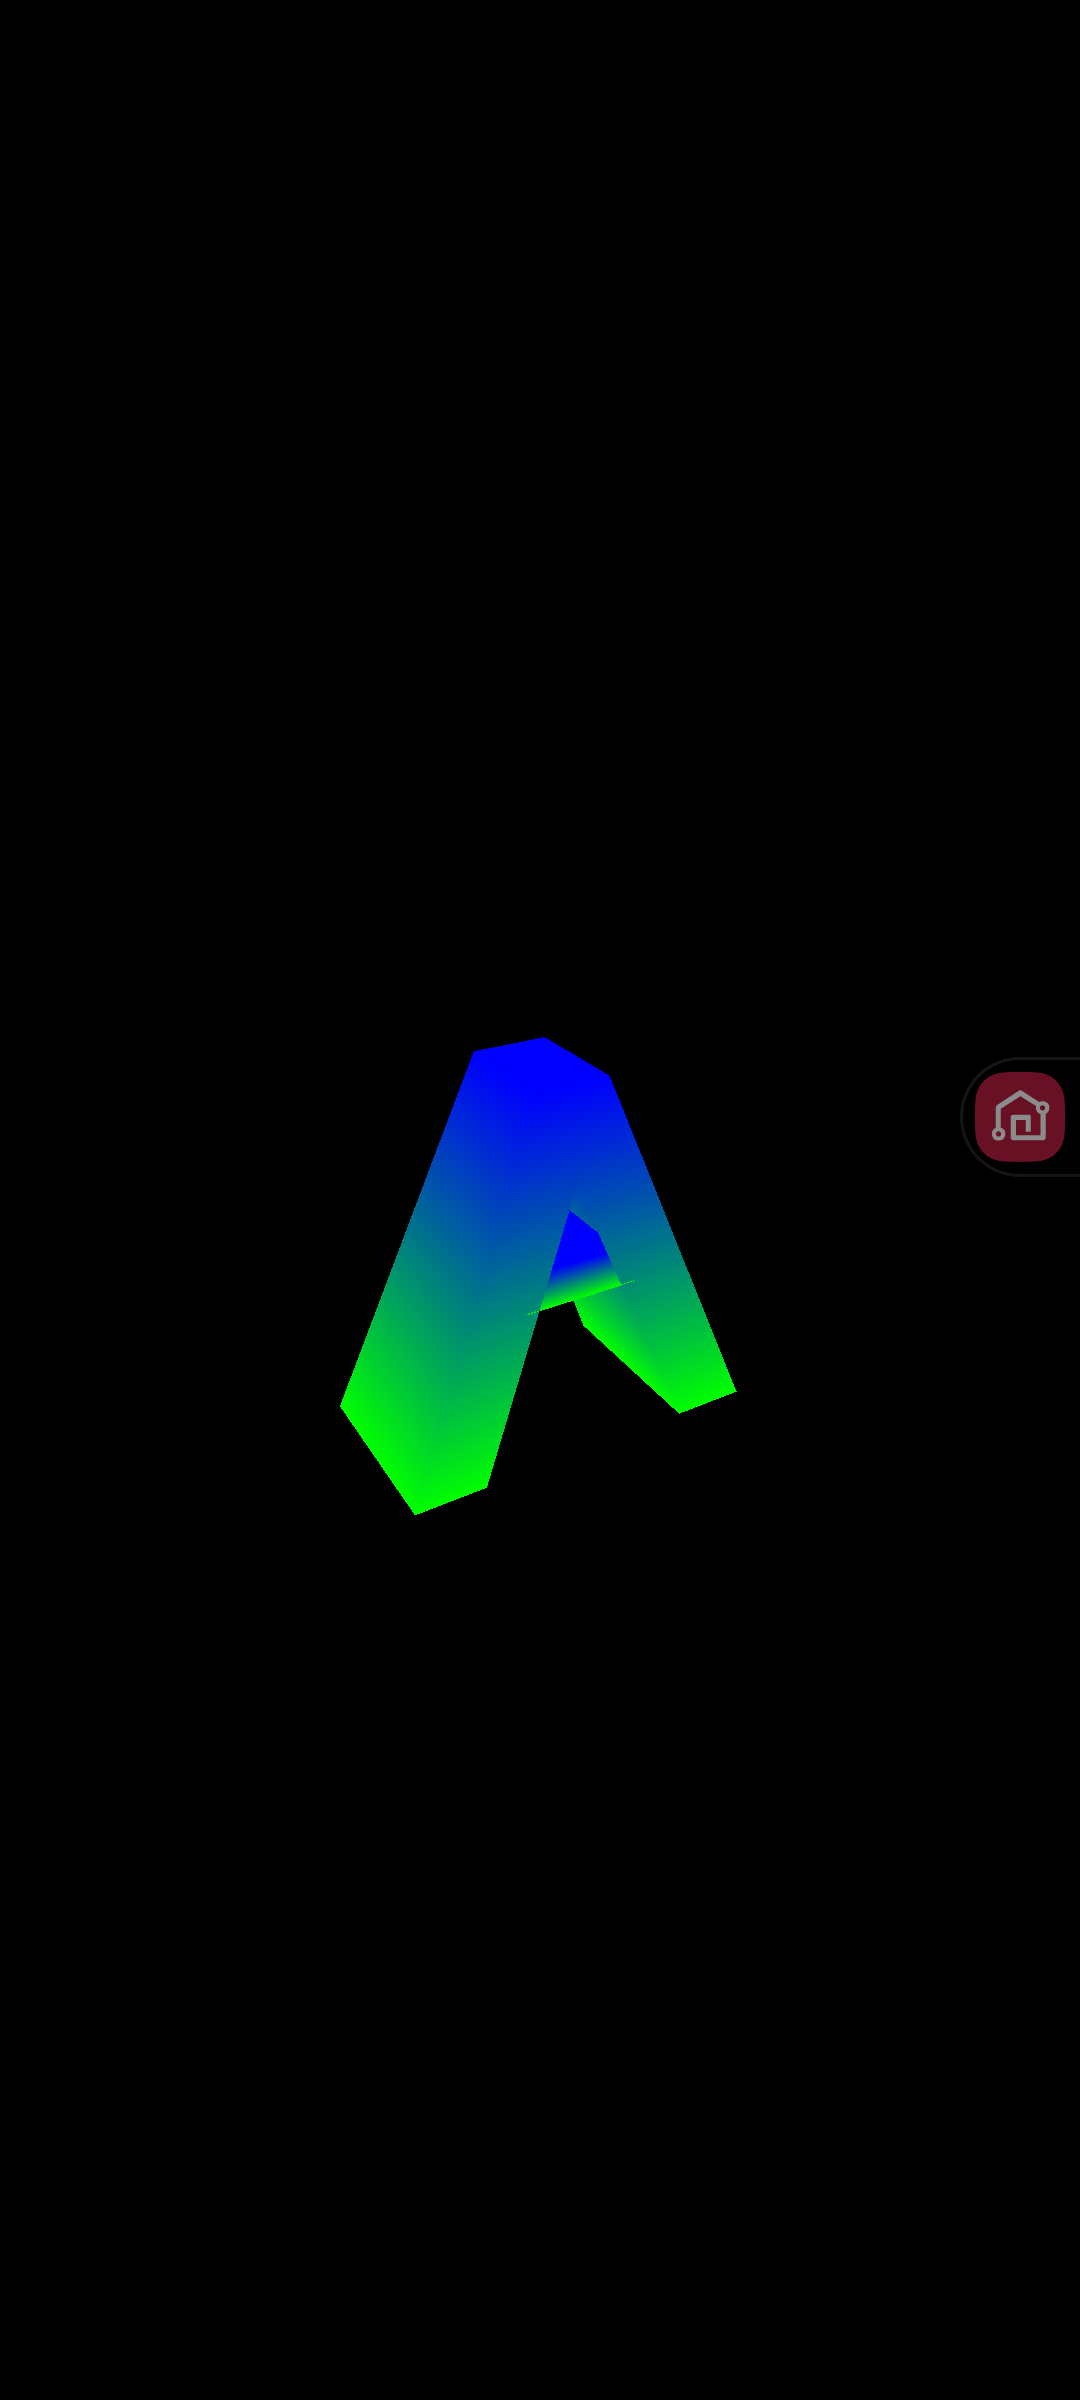
\includegraphics[width=1.0\linewidth]{PantallazosDemoTaller/Demo4.png}
\end{center}
\end{column}
\end{columns}


\end{frame}




\begin{frame}{Objetos 3D Complejos en OpenGL (2)}
\begin{columns}
\begin{column}{0.7\textwidth}

\begin{itemize}
\item Es posible dibujar objetos compuestos de múltiples triángulos
\end{itemize}
\begin{block}{Demo \#5: Cilindro Multicolores}
\begin{itemize}
\item Sustituir el MainActivity.java del proyecto con el MainActivity de la carpeta del demo
\item Copiar los archivos MyGLSurfaceRenderer.java y MyGLSurfaceView.java en la carpeta del package
\end{itemize}
\end{block}
\end{column}
\begin{column}{0.3\textwidth}
\begin{center}
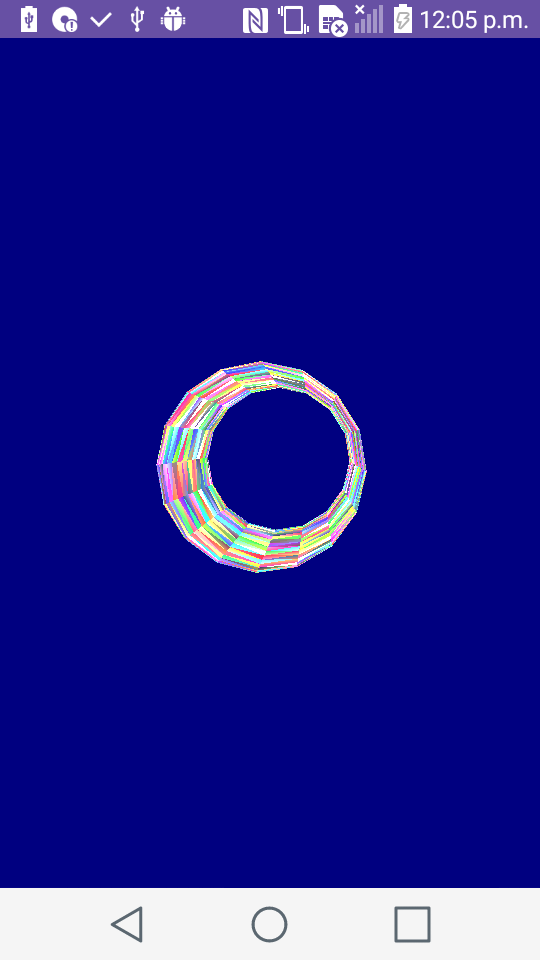
\includegraphics[width=1.0\linewidth]{PantallazosDemoTaller/Demo5.png}
\end{center}
\end{column}
\end{columns}


\end{frame}






\begin{frame}{Transformaciones}
\begin{columns}
\begin{column}{0.5\textwidth}
\begin{itemize}
\item \textbf{Translación.} Es un cambio en la posición de los objetos en cualquiera de los ejes.
\item \textbf{Escalamiento.} Es un cambio en el tamaño de un objeto con respecto a sus dimensiones en cualquiera de los ejes. 
\item \textbf{Rotación.} La orientación de un objeto puede ser cambiada mediante un ángulo de rotación.

\end{itemize}
\end{column}
\begin{column}{0.5\textwidth}
\begin{center}
% 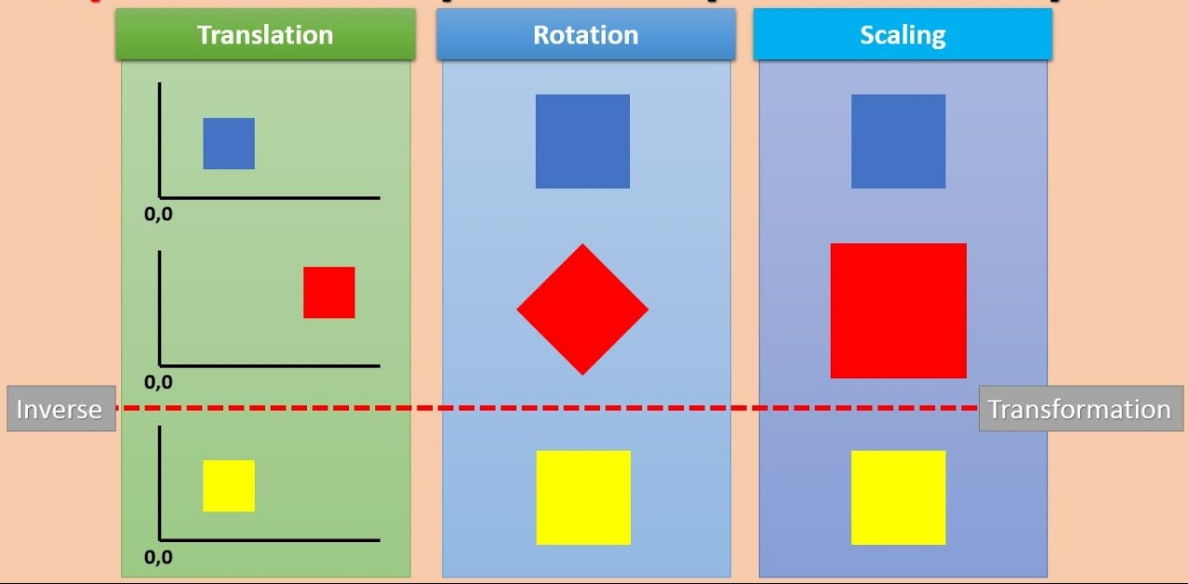
\includegraphics[width=0.8\textwidth]{FigsOpenGL/Transformaciones2D}
 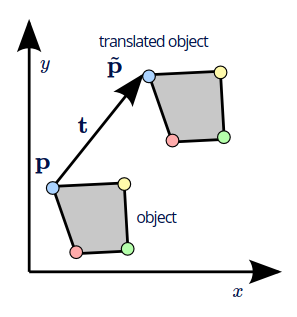
\includegraphics[width=0.45\textwidth]{FigsOpenGL/Traslacion}
     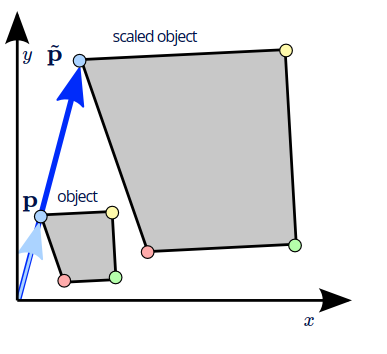
\includegraphics[width=0.52\textwidth]{FigsOpenGL/Escalamiento}\\
  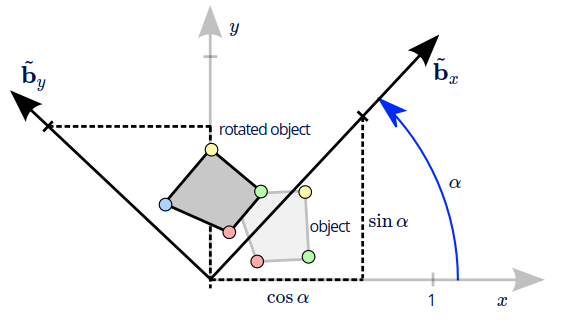
\includegraphics[width=0.7\textwidth]{FigsOpenGL/Rotacion}

 \end{center}
\end{column}
\end{columns}

\end{frame}


\begin{frame}{Aplicando Transformaciones en OpenGL}
\begin{columns}
\begin{column}{0.7\textwidth}

%\begin{itemize}
%\item Es posible dibujar objetos compuestos de múltiples triángulos
%\end{itemize}
\begin{block}{Demo \#6: Transformaciones}
\begin{itemize}
\item Sustituir el MainActivity.java del proyecto con el MainActivity de la carpeta del demo
\item Copiar el archivo LessonOneRenderer.java en la carpeta del package
\item Copiar el archivo \textit{activity\_main.xml} a la carpeta \textit{res/layout}
\end{itemize}
\end{block}
\end{column}
\begin{column}{0.3\textwidth}
\begin{center}
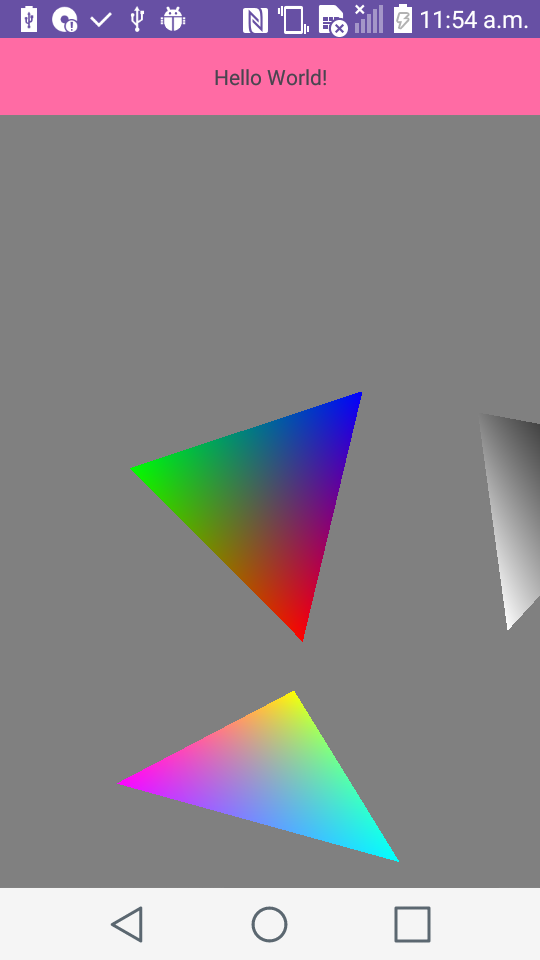
\includegraphics[width=1.0\linewidth]{PantallazosDemoTaller/Demo6.png}
\end{center}
\end{column}
\end{columns}


\end{frame}



\begin{frame}{Dibujar una esfera (1)}
\begin{columns}
\begin{column}{0.5\textwidth}
\begin{itemize}
\item La definición de esfera es una superficie cerrada en 3D donde cada punto de la esfera está a la misma distancia (radio) de un punto dado.
\item Dado que no podemos dibujar todos los puntos en una esfera, solo tomamos muestras de una cantidad limitada de puntos dividiendo la esfera por sectores (longitud) y pilas (latitud).
\end{itemize}

\end{column}
\begin{column}{0.5\textwidth}
\begin{center}
 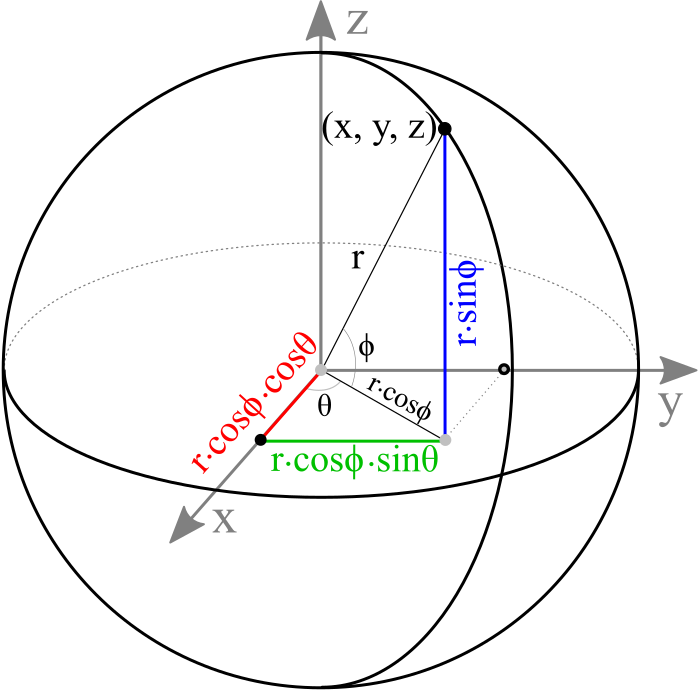
\includegraphics[width=0.8\textwidth]{FigsOpenGL/gl_sphere01}
 \end{center}
\end{column}
\end{columns}
\footnotetext{\url{http://www.songho.ca/opengl/gl_sphere.html}}


\end{frame}

\begin{frame}{Dibujar una esfera (2)}
\begin{columns}
\begin{column}{0.4\textwidth}
\begin{itemize}
\item Para dibujar la superficie de una esfera en OpenGL, debe triangular los vértices adyacentes para formar polígonos. Es posible usar una sola tira triangular para renderizar toda la esfera.
\item Cada sector de una pila requiere 2 triángulos.
\end{itemize}
%\begin{block}{Demo \#4}
%Esfera en OpenGL ES
%\end{block}

\end{column}
\begin{column}{0.3\textwidth}
\begin{center}
 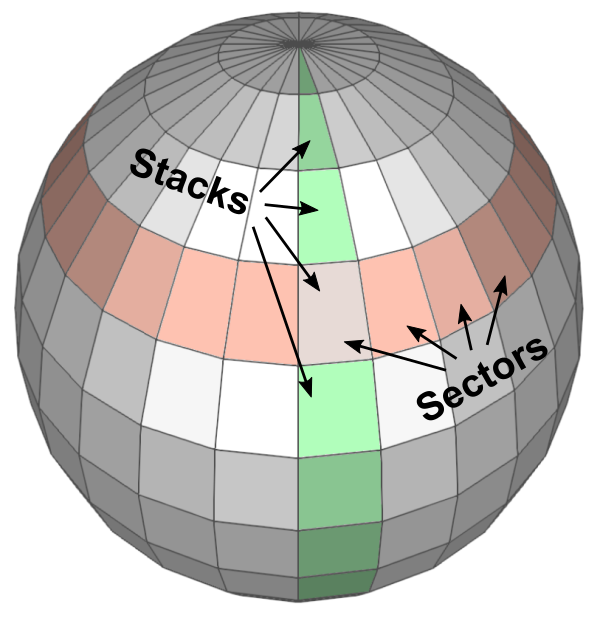
\includegraphics[width=0.98\textwidth]{FigsOpenGL/gl_sphere02}
 \end{center}

\end{column}
\begin{column}{0.3\textwidth}
\begin{center}
 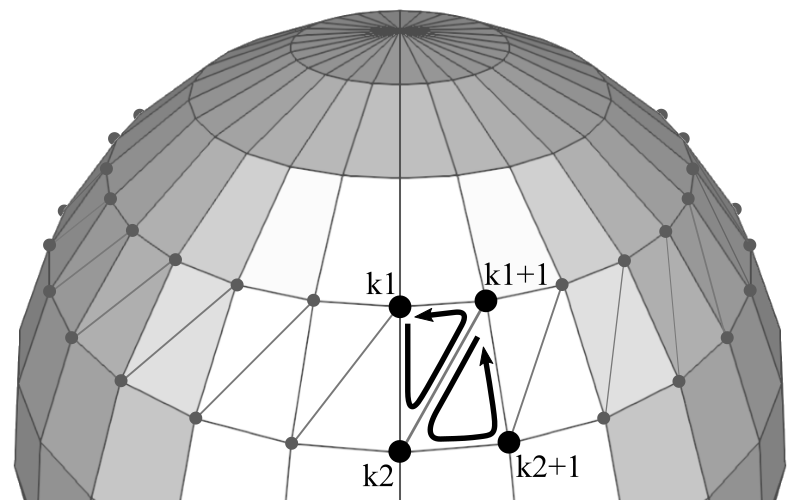
\includegraphics[width=0.98\textwidth]{FigsOpenGL/gl_sphere03}
 \end{center}
\end{column}
\end{columns}


\end{frame}



\begin{frame}{Esfera en OpenGL}
\begin{columns}
\begin{column}{0.7\textwidth}

%\begin{itemize}
%\item Es posible dibujar objetos compuestos de múltiples triángulos
%\end{itemize}
\begin{block}{Demo \#7: Esfera}
\begin{itemize}
\item Sustituir el MainActivity.java del proyecto con el MainActivity de la carpeta del demo
\item Copiar los archivos MyGLRenderer.java y MyGLSurfaceView.java en la carpeta del packag
\end{itemize}
\end{block}
\end{column}
\begin{column}{0.3\textwidth}
\begin{center}
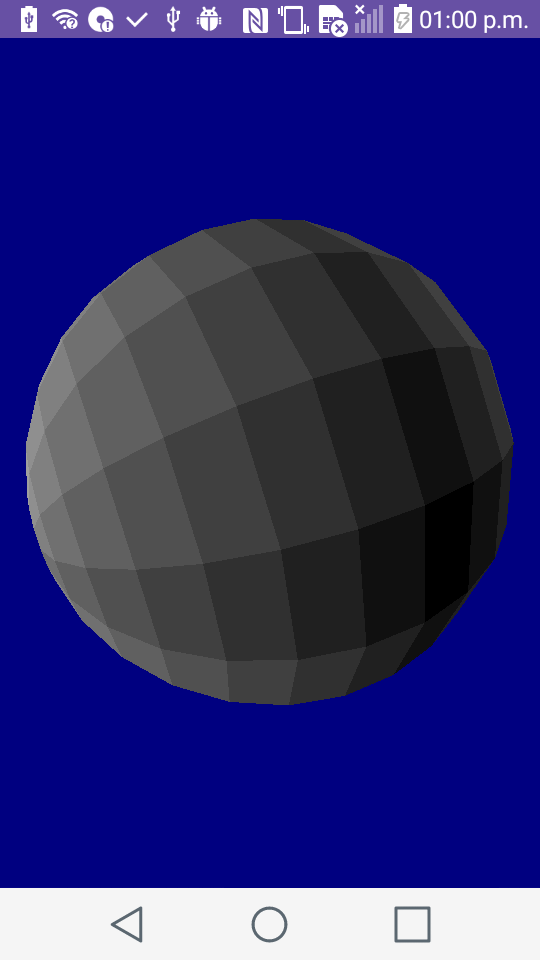
\includegraphics[width=1.0\linewidth]{PantallazosDemoTaller/Demo7.png}
\end{center}
\end{column}
\end{columns}


\end{frame}



\section{Texturas}
\begin{frame}{Mapeo de Texturas}
%\begin{block}{Demo \#5}
%Texturas en OpenGL
%\end{block}
\begin{columns}
\begin{column}{0.6\textwidth}
\begin{itemize}
\item El mapeo de texturas en gráficos por computadora se refiere a la aplicación de un tipo de superficie a una imagen 3D. 
%\item Una textura puede ser uniforme, como una pared de ladrillos, o irregular, como vetas de madera o mármol. 
\item El método común es crear una imagen de mapa de bits 2D de la textura, llamada \textit{mapa de textura}, que luego se \textit{envuelve} alrededor del objeto 3D. 
\item Para texturas mas precisas se emplean funciones matemáticas en lugar de mapas de bits.
\end{itemize}
%\begin{block}{Demo \#5}
%Texturas en OpenGL
%\end{block}
\end{column}
\begin{column}{0.4\textwidth}
    \begin{center}
         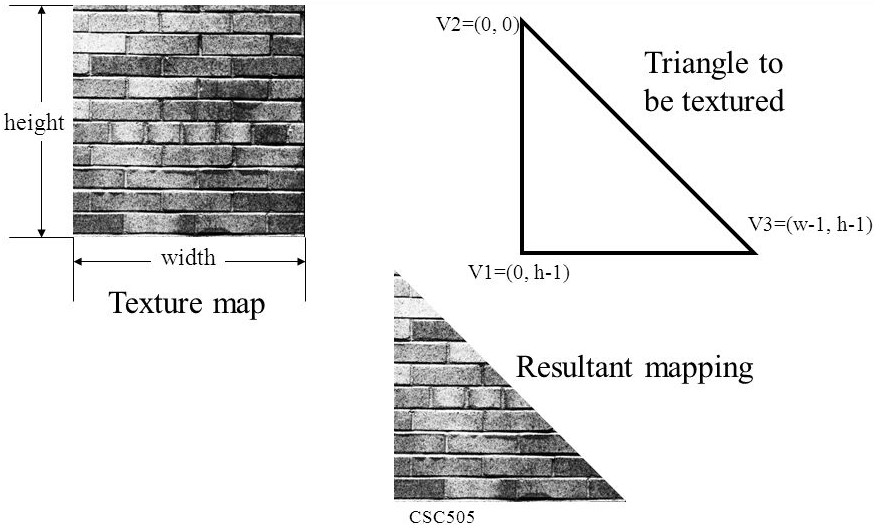
\includegraphics[width=0.98\textwidth]{FigsOpenGL/Textures}
     \end{center}
\end{column}
\end{columns}
\end{frame}



\begin{frame}{Textura en OpenGL}
\begin{columns}
\begin{column}{0.7\textwidth}
\begin{block}{Demo \#8: Textura en un Cubo}
\begin{itemize}
\item Sustituir el MainActivity.java del proyecto con el MainActivity de la carpeta del demo
\item Copiar los archivos BaseActivity.java, GLESChecker.java, ShaderHelper.java, Shape.java, ShapeRenderer.java. TextResourceReader.java, TextureHelper.java y TexturedCube.java en la carpeta del package
\item Crear una carpeta dentro de la carpeta res con nombre raw. Copiar dentro los archivos con extension glsl
\item Copiar las imágenes .png en la carpeta drawable 
\end{itemize}
\end{block}
\end{column}
\begin{column}{0.3\textwidth}
\begin{center}
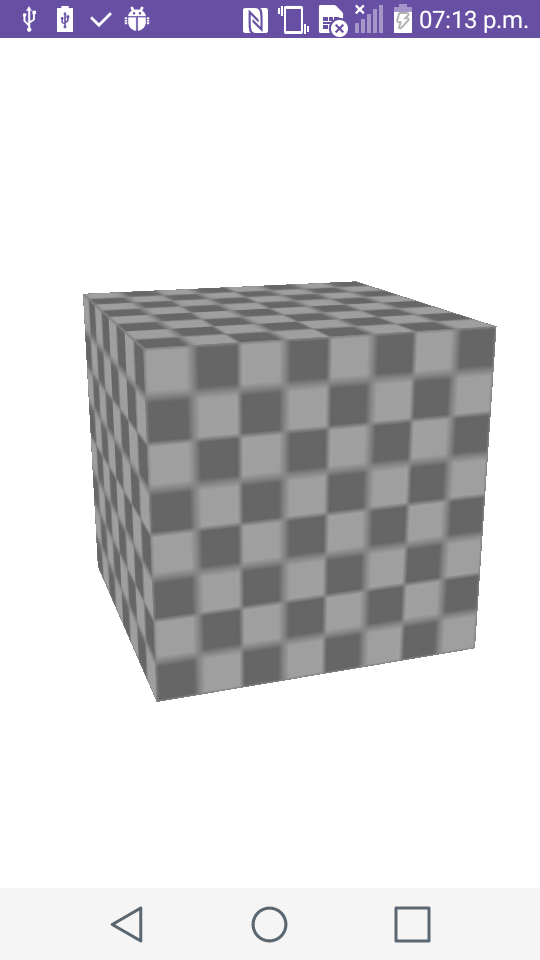
\includegraphics[width=1.0\linewidth]{PantallazosDemoTaller/Demo08.png}
\end{center}
\end{column}
\end{columns}


\end{frame}



\begin{frame}{Multiples Texturas en OpenGL}
%\begin{block}{Demo \#6}
%Multiples Texturas en OpenGL
%\end{block}
\begin{columns}
\begin{column}{0.5\textwidth}
\begin{itemize}
\item 
\end{itemize}
    \begin{center}
        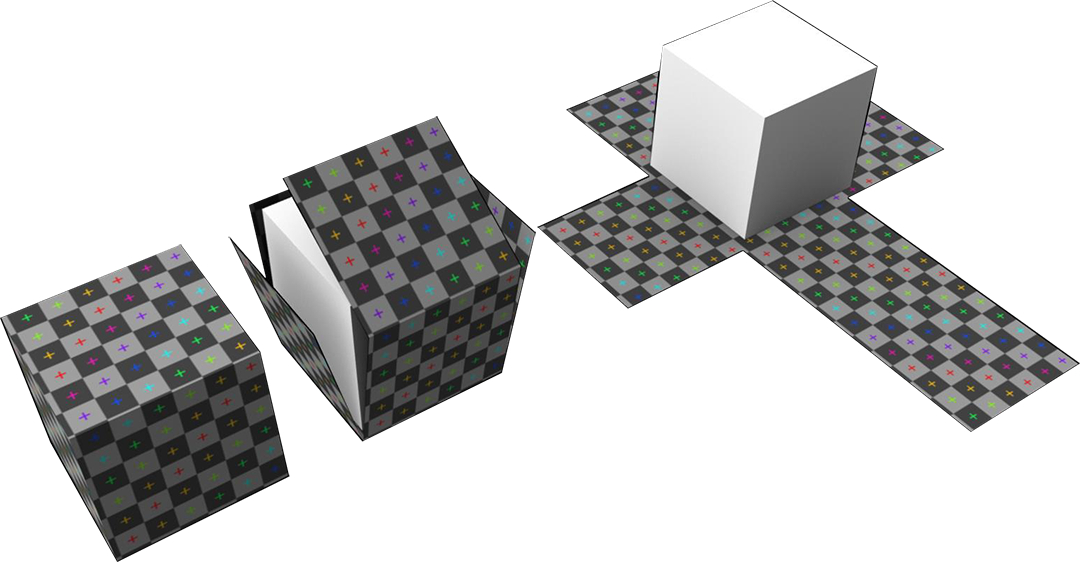
\includegraphics[width=0.98\textwidth]{FigsOpenGL/RefImgBoxmap2}
     \end{center}
%\begin{block}{Demo \#6}
%Multiples Texturas en OpenGL
%\end{block}
\end{column}
\begin{column}{0.5\textwidth}
    \begin{center}
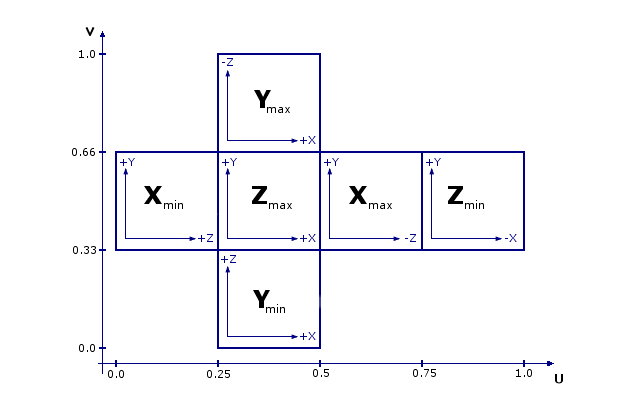
\includegraphics[width=0.98\textwidth]{FigsOpenGL/RefImgBoxmap}
%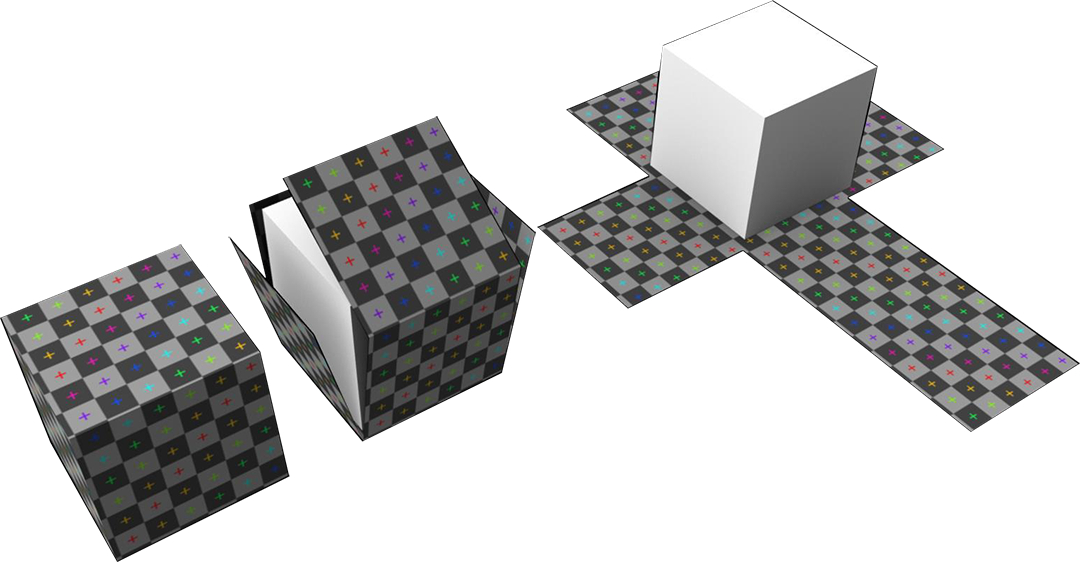
\includegraphics[width=0.98\textwidth]{FigsOpenGL/RefImgBoxmap2}
     \end{center}
\end{column}
\end{columns}

\end{frame}



\begin{frame}{Multiples Texturas en OpenGL}
\begin{columns}
\begin{column}{0.7\textwidth}
\begin{block}{Demo \#9: Multiples Texturas en un Cubo}
\begin{itemize}
\item Sustituir el \textit{MainActivity.java} del proyecto con el \textit{MainActivity} de la carpeta del demo
\item Copiar los archivos \textit{BaseActivity.java, GLESChecker.java, MultiTexturedCube.java, ShaderHelper.java, Shape.java, ShapeRenderer.java. TextResourceReader.java, TextureHelper.java} y en la carpeta del package
\item Crear una carpeta dentro de la carpeta res con nombre \textit{raw}. Copiar dentro los archivos con extension \textit{.glsl}
\item Copiar las imágenes .png en la carpeta drawable 
\end{itemize}
\end{block}
\end{column}
\begin{column}{0.3\textwidth}
\begin{center}
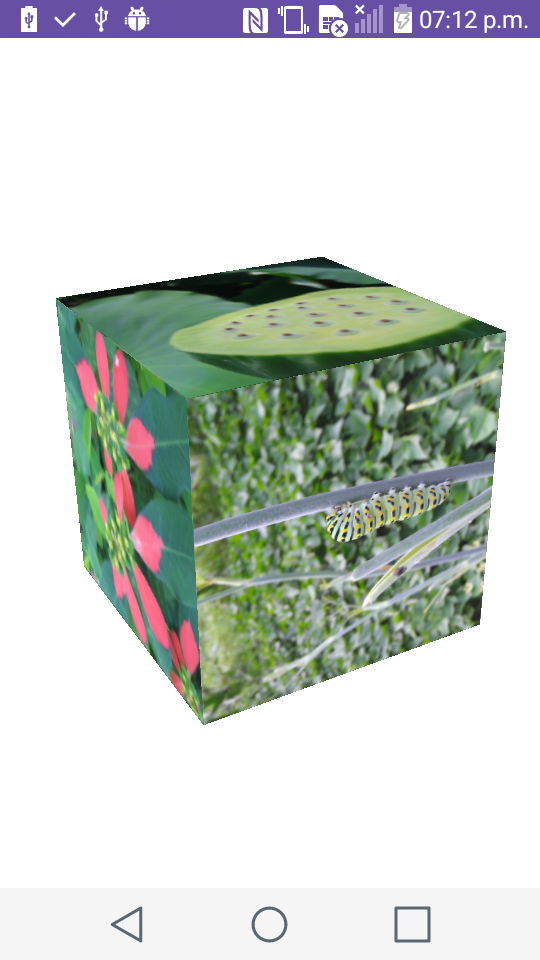
\includegraphics[width=1.0\linewidth]{PantallazosDemoTaller/Demo09.png}
\end{center}
\end{column}
\end{columns}


\end{frame}


\begin{frame}{UV mapping}
\begin{columns}
\begin{column}{0.5\textwidth}
\begin{itemize}
\item El mapeo UV es el proceso de modelado 3D de proyectar una imagen 2D en la superficie de un modelo 3D para el mapeo de texturas. Las letras $U$ y $V$ denotan los ejes de la textura 2D porque $X$, $Y$ y $Z$ ya se utilizan para denotar los ejes del objeto 3D en el espacio modelo,
\end{itemize}
\end{column}
\begin{column}{0.5\textwidth}
    \begin{center}
         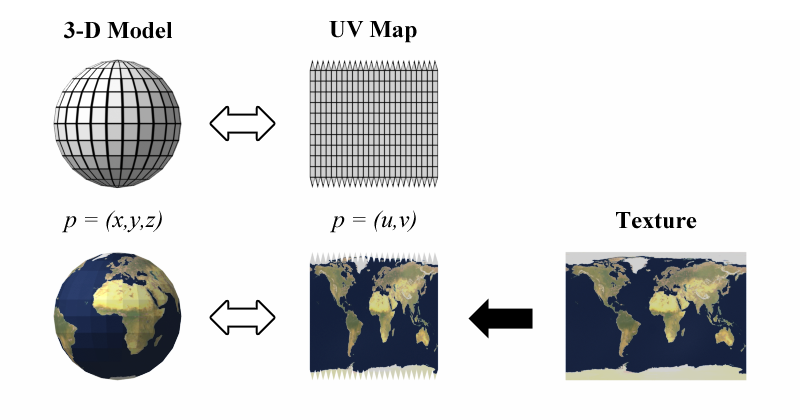
\includegraphics[width=0.98\textwidth]{FigsOpenGL/UVMapping}
     \end{center}
\end{column}
\end{columns}
\end{frame}


\begin{frame}{Textura sobre una esfera}
\begin{columns}
\begin{column}{0.7\textwidth}
\begin{block}{Demo \#10: Textura sobre una esfera}
\begin{itemize}
\item Sustituir el \textit{MainActivity.java} del proyecto con el \textit{MainActivity} de la carpeta del demo
\item Copiar los archivos \textit{BaseActivity.java, GLESChecker.java, Globe.java, ShaderHelper.java, Shape.java, ShapeRenderer.java. TextResourceReader.java y TextureHelper.java} en la carpeta del package
\item Crear una carpeta dentro de la carpeta res con nombre \textit{raw}. Copiar dentro los archivos con extension \textit{.glsl}
\item Copiar las imágenes .png en la carpeta drawable 
\end{itemize}
\end{block}
\end{column}
\begin{column}{0.3\textwidth}
\begin{center}
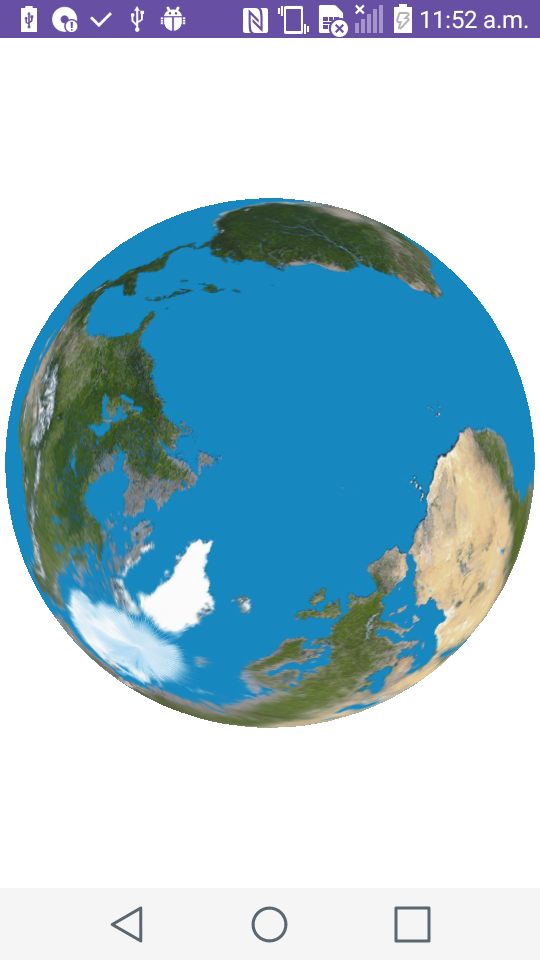
\includegraphics[width=1.0\linewidth]{PantallazosDemoTaller/Demo10.png}
\end{center}
\end{column}
\end{columns}
\end{frame}




\section[Iluminación]{Iluminación y Sombreado}
\begin{frame}{Iluminación Ambiente y Difusa}
\begin{columns}
\begin{column}{0.5\textwidth}
\begin{itemize}
\item Iluminación ambiental: lo que los objetos nunca están completamente oscuros. 
\item Iluminación difusa: simula el impacto direccional que tiene un objeto ligero sobre un objeto. 
\item Iluminación especular: simula el punto brillante (del color de la fuente) de una luz que aparece sobre objetos brillantes.
\end{itemize}
\end{column}
\begin{column}{0.5\textwidth}
\begin{center}
 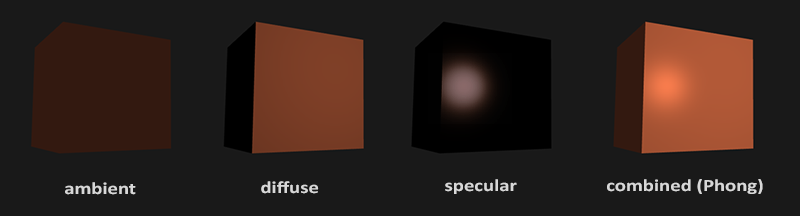
\includegraphics[width=0.98\textwidth]{FigsOpenGL/basic_lighting_phong}\\
 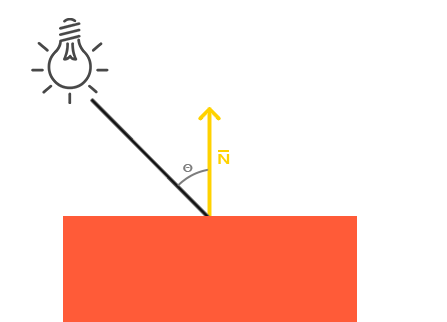
\includegraphics[width=0.48\textwidth]{FigsOpenGL/diffuse_light}
 \end{center}
\end{column}
\end{columns}
%\begin{block}{Demo \#8}
%Iluminacion Ambiente y Difusa
%\end{block}
\end{frame}

\begin{frame}{Demos de Iluminación (1)}
\begin{columns}
\begin{column}{0.7\textwidth}
\begin{block}{Demo \#11: Iluminación por Vertices}
\begin{itemize}
\item Sustituir el \textit{MainActivity.java} del proyecto con el \textit{MainActivity} de la carpeta del demo
\item Copiar el archivo \textit{LessonTwoRenderer.java} en la carpeta del package
%\item Crear una carpeta dentro de la carpeta res con nombre \textit{raw}. Copiar dentro los archivos con extension \textit{.glsl}
%\item Copiar las imágenes .png en la carpeta drawable 
\end{itemize}
\end{block}
\end{column}
\begin{column}{0.3\textwidth}
\begin{center}
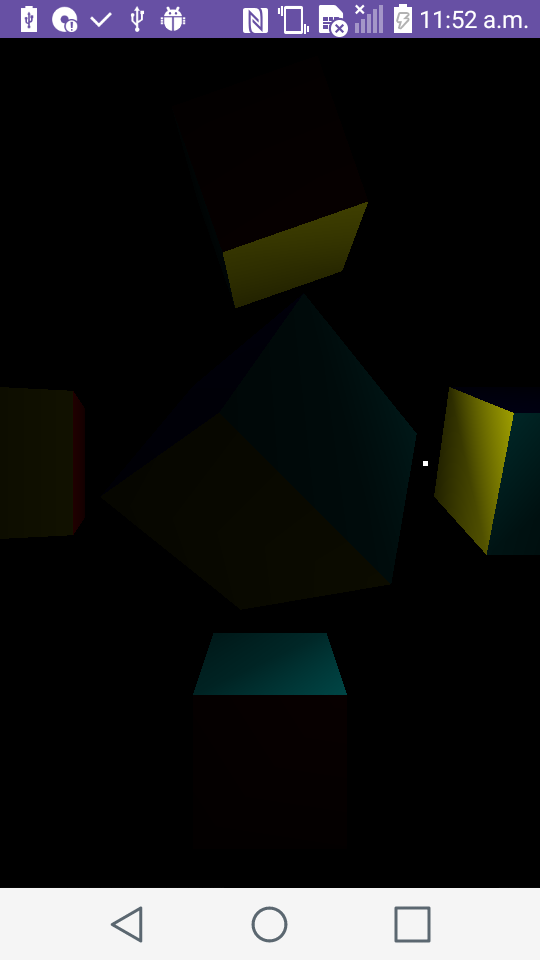
\includegraphics[width=1.0\linewidth]{PantallazosDemoTaller/Demo11.png}
\end{center}
\end{column}
\end{columns}
\end{frame}



%\section{Iluminación y Sombreado}
\begin{frame}{Iluminación por Fragmentos}
\begin{columns}
\begin{column}{0.5\textwidth}
\begin{itemize}
\item En la iluminación por vértice, la cara frontal del cubo muestra un sombreada plana sin evidencia de indicencia de luz. Los cuatro puntos de la cara frontal son equidistantes de la luz, y intensidad en cada puntos es interpolada mediante los triángulos que forman la cara frontal.
\item En la iluminación por fragmento hay un efecto mucho más notorio en la misma cara del cubo.
\end{itemize}
%\begin{block}{Demo \#9}
%Iluminación por Fragmentos
%\end{block}

\end{column}
\begin{column}{0.5\textwidth}
\begin{center}
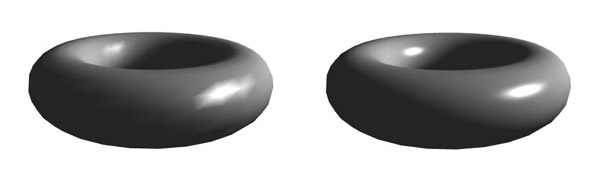
\includegraphics[width=0.48\textwidth]{FigsOpenGL/specular3}\\
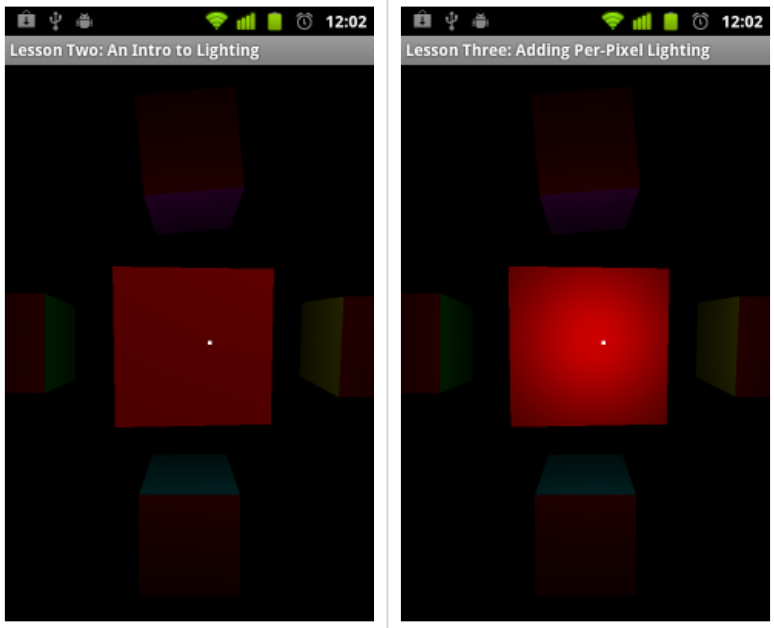
\includegraphics[width=0.78\textwidth]{FigsOpenGL/PerPixelVsPerFragmentShading}
 \end{center}
\end{column}
\end{columns}

\end{frame}

\begin{frame}{Demos de Iluminación (2)}
\begin{columns}
\begin{column}{0.7\textwidth}
\begin{block}{Demo \#12: Iluminación por Fragmentos}
\begin{itemize}
\item Sustituir el \textit{MainActivity.java} del proyecto con el \textit{MainActivity} de la carpeta del demo
\item Copiar los archivos \textit{LessonTwoRenderer.java y LessonThreeRenderer.java} en la carpeta del package
%\item Crear una carpeta dentro de la carpeta res con nombre \textit{raw}. Copiar dentro los archivos con extension \textit{.glsl}
%\item Copiar las imágenes .png en la carpeta drawable 
\end{itemize}
\end{block}
\end{column}
\begin{column}{0.3\textwidth}
\begin{center}
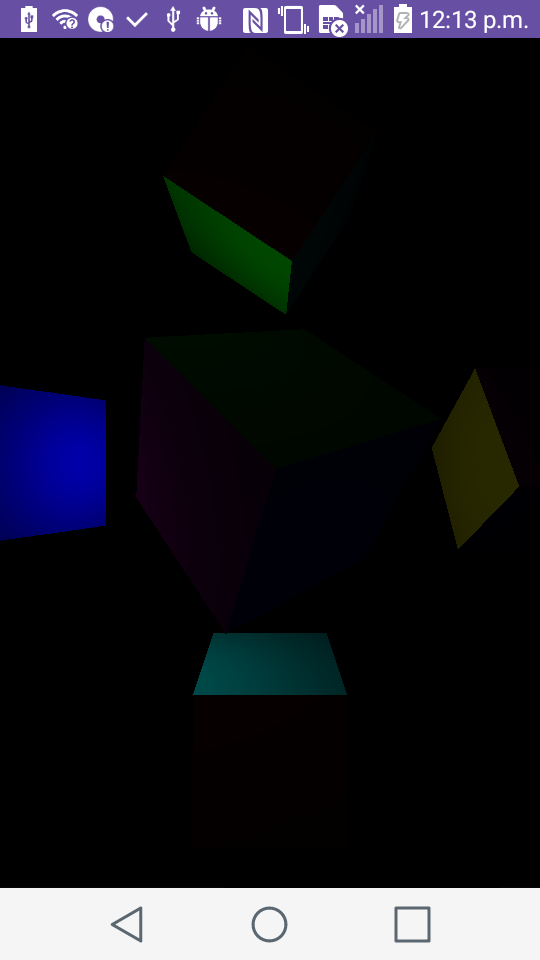
\includegraphics[width=1.0\linewidth]{PantallazosDemoTaller/Demo12.png}
\end{center}
\end{column}
\end{columns}
\end{frame}



\begin{frame}{Textura e Iluminación}
\begin{columns}
\begin{column}{0.5\textwidth}
\begin{itemize}
\item Mapear texturas permite construir ambientes 3D de apariencia realista. 
\item Para lograr esto, es necesario enviar al \textit{Vertex Shader} una matriz con información de coordenadas de textura. 
\item Para agregar realismo a las escenas, es necesario combinar texturas más iluminación, siendo requerido un código más complejo en el \textit{Fragment Shader} para lograr dicha tarea. 
\end{itemize}
\end{column}
\begin{column}{0.5\textwidth}
\begin{center}
% 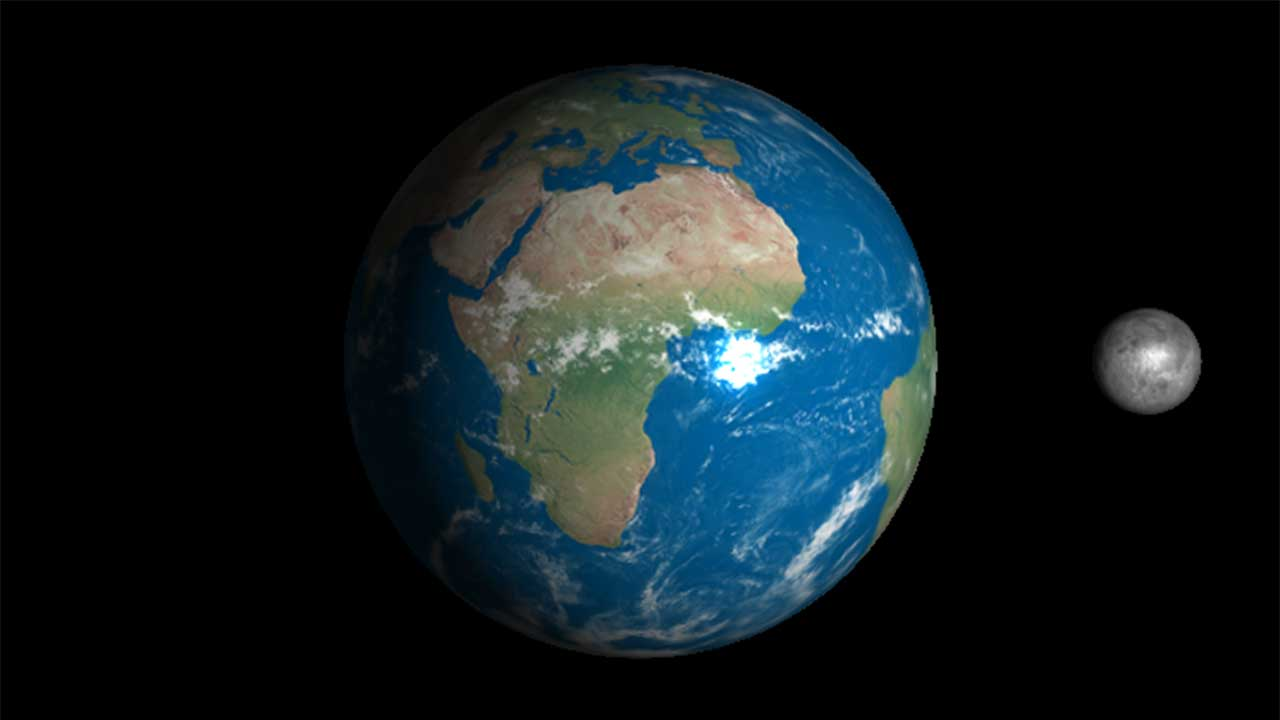
\includegraphics[width=0.98\textwidth]{FigsOpenGL/OpenGL_TexturingAndLighting}
 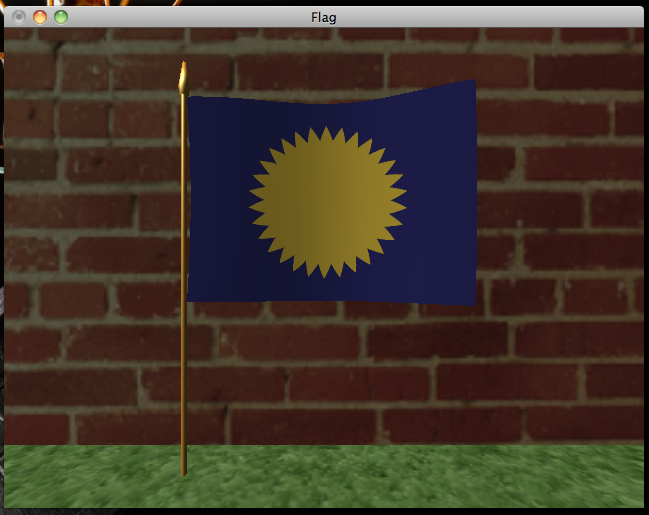
\includegraphics[width=0.98\textwidth]{FigsOpenGL/Textura_e_Iluminacion}
\end{center}
\end{column}
\end{columns}

\end{frame}


\begin{frame}{Textura e Iluminación}
\begin{columns}
\begin{column}{0.7\textwidth}
\begin{block}{Demo \#13: Textura e Iluminación sobre una Esfera}
\begin{itemize}
\item Sustituir el \textit{MainActivity.java} del proyecto con el \textit{MainActivity} de la carpeta del demo
\item Copiar los archivos \textit{BaseActivity.java, GLESChecker.java, ShaderHelper.java, Shape.java, ShapeRenderer.java, Shere.java, TextResourceReader.java y TextureHelper.java} en la carpeta del package
\item Crear una carpeta dentro de la carpeta \textit{res} con nombre \textit{raw}. Copiar dentro los archivos con extension \textit{.glsl}
\item Copiar las imágenes .png en la carpeta drawable 
\end{itemize}
\end{block}
\end{column}
\begin{column}{0.3\textwidth}
\begin{center}
\includegraphics[width=1.0\linewidth]{PantallazosDemoTaller/Demo13.png}
\end{center}
\end{column}
\end{columns}
\end{frame}



\section[RV]{Realidad Virtual}
\begin{frame}[fragile]
\frametitle{Realidad Virtual OpenGLES Android}
\begin{itemize}
\item Para este demo, es necesario contar con un teléfono de gama media hacia arriba, que incluye sensores de movimiento (acelerómetros y giroscopios)
\item De manera opcional, se puede utilizar el adaptador de realidad virtual para una interacción inmersiva
\end{itemize}
\end{frame}


\begin{frame}[fragile]
\frametitle{Realidad Virtual OpenGLES Android}
%\begin{columns}
%\begin{column}{0.99\textwidth}
\begin{block}{Demo \#14: Realidad Virtual (1)}
\begin{itemize}
\item Sustituir el \textit{MainActivity.java} del proyecto con el \textit{MainActivity} de la carpeta del demo
\item Copiar \textbf{todos} los archivos .java de la carpeta a \textbf{EXCEPCION} de \textit{ExampleInstrumentedTest.java y ExampleUnitTest.java} en la carpeta del package
\item Crear una carpeta dentro de la carpeta \textit{res} con nombre \textit{raw}. Copiar dentro los archivos con extension \textit{.shader}
\item Agregar la siguiente linea a la sección dependencias del archivo build.gradle.kts: 

\begin{minted}[fontsize=\tiny]{java}
implementation ("com.google.protobuf.nano:protobuf-javanano:3.0.0-alpha-2")
\end{minted}
\end{itemize}
\end{block}
\end{frame}


\begin{frame}[fragile]
\frametitle{Realidad Virtual OpenGLES Android}
\begin{block}{Demo \#14: Realidad Virtual (2)}
\begin{itemize}
\item Agregar los siguientes permisos al archivo Android Manifest
\begin{minted}[highlightlines={2,10,13-17},linenos,fontsize=\tiny]{xml}
    <uses-feature android:name="android.hardware.sensor.accelerometer" android:required="true"/>
    <uses-feature android:name="android.hardware.sensor.gyroscope" android:required="true"/>
    <uses-permission android:name="android.permission.HIGH_SAMPLING_RATE_SENSORS"/>
    <uses-permission android:name="android.permission.NFC" />
    <uses-permission android:name="android.permission.VIBRATE" />
    <uses-feature android:glEsVersion="0x00020000" android:required="true" />
\end{minted}
\end{itemize}
\end{block}
\end{frame}

\begin{frame}[fragile]
\frametitle{Realidad Virtual OpenGLES Android}
%\begin{columns}
%\begin{column}{0.99\textwidth}
\begin{block}{Demo \#14: Realidad Virtual (3)}
\begin{itemize}
\item Reemplazar el \textit{activity\_main.xml}, cambiando por package de su proyecto (lineas resaltadas):
\begin{minted}[highlightlines={12,16},linenos,fontsize=\tiny]{xml}
<?xml version="1.0" encoding="utf-8"?>
<LinearLayout xmlns:android="http://schemas.android.com/apk/res/android"
    android:id="@+id/ui_layout"
    android:orientation="vertical"
    android:layout_width="match_parent"
    android:layout_height="match_parent" >
    <LinearLayout
        android:layout_width="match_parent"
        android:orientation="horizontal"
        android:layout_weight="5"
        android:layout_height="0dp">
        <com.example.realidadvirtual_2023.CardboardView
            android:id="@+id/cardboard_view"
            android:layout_width="match_parent"
            android:layout_height="match_parent"/>
        <com.example.realidadvirtual_2023.CardboardOverlayView
            android:id="@+id/overlay"
            android:layout_width="match_parent"
            android:layout_height="match_parent" />
    </LinearLayout>
    <!-- ESte panel es temporal, solo para depuracion -->
\end{minted}
\end{itemize}
\end{block}
\end{frame}


\begin{frame}[fragile]
\frametitle{Realidad Virtual OpenGLES Android}
\begin{columns}
\begin{column}{0.48\textwidth}
\begin{itemize}
\item La vista es afectada por los sensores del telefono (acelerómetros y giroscopios)
\item La posición en el plano XZ es afectada por los botones ubicados en la parte inferior
\end{itemize}
\end{column}
\begin{column}{0.48\textwidth}
\includegraphics[width=0.99\linewidth]{PantallazosDemoTaller/Pantallazo1.png}
\includegraphics[width=0.99\linewidth]{PantallazosDemoTaller/Pantallazo2.png}
\end{column}
\end{columns}
\end{frame}



\section[OpenCV y RA]{OpenCV y Realidad Aumentada}
\begin{frame}[fragile]
\frametitle{OpenCV en Android}
\begin{block}{Demo \#15: OpenCV Android - Parte I (1)}
\begin{itemize}
\item Descomprimir la carpeta opencv-4.8.0-android-sdk.zip y copiar la carpeta sdk a la carpeta raiz del proyecto Android
\item Editar Manualmente el archivo build.gradle de la carpeta SDK y hacer los siguiente cambios: 
\begin{itemize}
\item Comentar las siguientes lienas:
\begin{minted}[fontsize=\tiny]{java}
apply plugin: 'com.android.library'
apply plugin: 'kotlin-android'
\end{minted}
\item E inmediatamente abajo agregar la siguiente linea:
\begin{minted}[fontsize=\tiny]{java}
plugins { id("com.android.library") }
\end{minted}
\item Agregar la siguiente linea dentro de android \{ ... \}
\begin{minted}[fontsize=\tiny]{java}
namespace "org.opencv"
\end{minted}
\item Dentro del grupo android \{ \} - Cambiar el numero despues de compileSdkVersion y targetSdkVersion a 33
\begin{minted}[fontsize=\tiny]{java}
compileSdkVersion 33
targetSdkVersion 33
\end{minted}
\end{itemize}
\end{itemize}
\end{block}
\end{frame}



\begin{frame}[fragile]
\frametitle{OpenCV en Android}
\begin{block}{Demo \#15: OpenCV Android - Parte I (2)}
\begin{itemize}
\item Dentro del grupo android \{ \}, agregar lo siguiente:
\begin{minted}[fontsize=\tiny]{java}
    buildFeatures {
        aidl = true
        buildConfig = true
    }
\end{minted}
\item Agregar las sigueintes lineas al final del settings.graddle.kts (Sustituir por la ruta donde esta la carpeta SDK dentro del proyecto)
\begin{minted}[fontsize=\tiny]{java}
include(":sdk")
project(":sdk").projectDir = File("/home/marco/AndroidStudioProjects/OpenCV_JavaFin5/sdk")
\end{minted}

\item Agregar al archivo \textit{gradle.properties} la siguiente linea
\begin{minted}[fontsize=\tiny]{java}
android.defaults.buildfeatures.buildconfig=true
\end{minted}

\item Agregar en la seccion dependencias del archivo \textit{build.gradle.kts (Module:app)} la siguiente linea:
\begin{minted}[fontsize=\tiny]{java}
implementation(project(mapOf("path" to ":sdk")))
\end{minted}
\end{itemize}
\end{block}
\end{frame}


\begin{frame}[fragile]
\frametitle{OpenCV en Android}
\begin{block}{Demo \#15: OpenCV Android  - Parte I (3)}
\begin{itemize}

\item Agregar las siguientes lineas dentro del onCreate del Main Activity
\begin{minted}[fontsize=\tiny]{java}
if (OpenCVLoader.initDebug()) {
            Toast.makeText(getApplicationContext(),"OpenCV loaded"+OpenCVLoader.OPENCV_VERSION,Toast.LENGTH_SHORT).show();
        }
\end{minted}
\item Para corregir el error sobre la palabra \textit{OpenCVLoader}, ubiquen el cursor el dicha palabra y presione la combinación ALT + ENTER. En la primera opción debe agregar el import a la sección de imports del proyecto.
\item Repetir el paso anterior para la palabra \textit{Toast}.
\item Al ejecutar la aplicación, debe aparecer un mensaje que confirma que OpenCV fue cargado (con la versión específica descargada)
\end{itemize}
\end{block}
\end{frame}


\begin{frame}[fragile]
\frametitle{OpenCV en Android}
\begin{block}{Demo \#15: OpenCV Android  - Parte 2 (1)}
\begin{itemize}

\item Agregar las siguientes lineas al archivo \textit{AndroidManifest.xml}:
\begin{minted}[fontsize=\tiny]{xml}
   <uses-permission android:name="android.permission.CAMERA"/>
    <uses-feature android:name="android.hardware.camera" android:required="false"/>
    <uses-feature android:name="android.hardware.camera.autofocus" android:required="false"/>
    <uses-feature android:name="android.hardware.camera.front" android:required="false"/>
    <uses-feature android:name="android.hardware.camera.front.autofocus" android:required="false"/>
\end{minted}
\item Agregar el archivo \textit{color\_blob\_detection\_surface\_view} al la carpeta \textit{res/layout}
\item Agregar los archivos \textit{CubeRenderer.java, Cube.java, ColorBlobDetection.java} a la carpeta del Package
\item Sustitir el archivo \textit{MainActivity} del proyecto por el ubicado en la Carpeta
\end{itemize}
\end{block}
\end{frame}


\begin{frame}[fragile]
\frametitle{OpenCV en Android}
\begin{columns}
\begin{column}{0.48\textwidth}
\begin{itemize}
\item La vista es afectada por los sensores del telefono (acelerómetros y giroscopios)
\item La posición en el plano XZ es afectada por los botones ubicados en la parte inferior
\end{itemize}
\end{column}
\begin{column}{0.48\textwidth}
\includegraphics[width=0.99\linewidth]{PantallazosDemoTaller/Demo15-1.png}
\includegraphics[width=0.99\linewidth]{PantallazosDemoTaller/Demo15-2.png}
\end{column}
\end{columns}

\end{frame}



\begin{frame}[fragile]
\frametitle{Realidad Aumentada en Android}
%\begin{columns}
%\begin{column}{0.99\textwidth}
\begin{block}{Demo \#16: Realidad Aumentada en Kotlin}

\begin{itemize}
\item Se debe crear un proyecto NUEVO, pero seleccionar Kotlin como lenguaje
\item Agregar la siguiente linea a la sección dependencias del archivo build.gradle.kts y sincronizar el proyecto: 
\begin{minted}[fontsize=\tiny]{java}
implementation ("io.github.sceneview:arsceneview:0.9.0")
\end{minted}
\item Sustituir el MainActivity.kt del proyecto con el MainActivity de la carpeta del demo
\item Copiar el archivo \textit{activity\_main.xml} a la carpeta \textit{res/layout}
\item Copiar los archivos \textit{ic\_add.xml e ic\_anchor.xml} a la carpeta \textit{res/drawable}
\item Buscar superficie con textura (aparecera una matriz de puntos) $\rightarrow$ Place Object $\rightarrow$ New Object $\rightarrow$ Place Object
\end{itemize}

\end{block}
\end{frame}



\begin{frame}[fragile]
\frametitle{Realidad Aumentada en Android}
\begin{columns}
\begin{column}{0.48\textwidth}
\begin{itemize}
\item El objeto es fijado a la superficie texturizada seleccionada por el usuario
\item A partir de los sensores del teléfono, se cambia la vista manteniendo el objeto ``fijo'' a la superficie
\item Es posible agregar otros objetos (estan en formato GLB)

\end{itemize}
\end{column}
\begin{column}{0.48\textwidth}
\includegraphics[width=0.45\linewidth]{PantallazosDemoTaller/Demo16-1.png}
\includegraphics[width=0.45\linewidth]{PantallazosDemoTaller/Demo16-2.png}
\end{column}
\end{columns}
\end{frame}





\section[Conclusiones]{Conclusiones parte 2}
\begin{frame}{Conclusiones}
Recapitulando lo visto en esta presentación
\begin{itemize}
\item Revisamos conceptos relacionados con OpenGL, GLSL, CPUs, GPUs
\item Explicamos primitivas 2D, 3D, y se desarrollaron prototipos para su implementación
\item Comprendimos los diferentes modelos de iluminacion
\item Integramos graficos 2D con una aplicación de Realidad Virtual simple
\item Integramos graficos 2D con una aplicación de Realidad Aumentada simple
\end{itemize}
\end{frame}





\end{document}

